\documentclass{ieeeaccess}
\usepackage{cite}
\usepackage{amsmath,amssymb,amsfonts,mathtools,bm}
\usepackage{graphicx,array,booktabs,tabularx,siunitx,microtype}
\usepackage{xcolor}
\graphicspath{{figures/}}
\sisetup{detect-all=true}
\newcommand{\Svec}{\boldsymbol{S}}
\newcommand{\Avec}{\boldsymbol{A}}
\newcommand{\evec}{\boldsymbol{E}}
\newcommand{\mvec}{\boldsymbol{m}}
\newcommand{\cpx}{\mathrm{i}}
\newcommand{\Vroi}{\mathcal{V}_{\mathrm r}}
\newcommand{\norm}[1]{\left\lVert #1 \right\rVert}
\begin{document}
\doi{}
\history{}
\vol{--}
\year{--}
\title{Information-Aware Simulation and Verification of a Two-Face Microwave Stokes Analyser for a Rubidium-87 Atomic Receiver}
\author{\uppercase{Ryan N. Verghese}\authorrefmark{1}}
\address[1]{School of Engineering and Technology, University of New South Wales, Canberra, ACT, Australia}
\markboth{Verghese: Information-Aware Microwave Polarimetry for Rb-87 Atomic Receiver}{Verghese: Information-Aware Microwave Polarimetry for Rb-87 Atomic Receiver}
\begin{abstract}
Full-Stokes microwave polarimetry requires measurements sensitive to linear-field orientation and to the phase relation between orthogonal electric-field components. This work develops and evaluates a two layer, switch-programmable metasurface that supplies six polarisation-dependent measurements to a fixed receiving axis through electromagnetic simulation. Complex HFSS fields are converted into a six-by-four Stokes instrument whose rank, conditioning, received gain and information content determine the usefulness of its switching states. An analysis of 36 copper geometries increases the longest accepted sampled frequency bandwidth from 175 to 250 MHz. At 1.925 GHz, the selected periodic design yields rank four, a row-normalised condition number of 9.53 and 0.551\% disagreement between independently adapted meshes. An exhaustive switch-state analysis reveals strong differences in the information carried by individual states; under a declared fixed-time, equal-variance model, optimised dwell allocation reduces the inverse-trace uncertainty criterion by 40.8\%. A separate finite 3-by-3 HFSS study retains observability but exposes weaker circular sensitivity and mesh-dependent calibration transfer. The contribution is a reproducible simulation and measurement-basis design method, with explicit criteria for subsequent PCB and atomic-receiver validation.
\end{abstract}

\begin{keywords}
Full-stokes polarimetry, Microwave metasurfaces, HFSS electromagnetic simulation, Stokes instrument matrix conditioning, Switch-state optimization
\end{keywords}
\titlepgskip=-21pt
\maketitle
\section{Introduction}
An electromagnetic field carries information in magnitude and direction of its electric-field vector. Two microwave signals of equal frequency and power may therefore differ profoundly. One can be linearly polarised, while another traces an ellipse or reverses its circular handedness. A scalar Radio-Frequency (RF) receiver cannot resolve these distinctions. Recovering them requires a calibrated set of measurements that respond independently to the four Stokes parameters \cite{Azzam1988,Tyo2002,Goldstein2011}. The challenge is, therefore, obtaining those independent measurements from one practical receiving locus.

This problem arises naturally in Rydberg-atom sensing. In a Rubidium-87 vapour cell, optically interrogated transitions between highly excited states respond to a microwave field through Electromagnetically Induced Transparency (EIT) and Autler-Townes (AT) splitting \cite{Sedlacek2012,Sedlacek2013,Schlossberger2024,Verghese2026ICTON}. The optical system is a highly informative local field probe; however, one fixed atomic receiving axis does not itself identify an arbitrary incident polarisation. Here we investigate a different method: a switchable, dual-sided RF metasurface supplies the independent electromagnetic projections, while the atomic readout is treated as a separate transfer function.

The resulting design problems are as follows. Which copper geometry and switch configurations yield independent complex-field responses? How robustly can the Stokes vector be inferred from them? Can those responses survive finite-panel boundaries, unequal received gain and realistic acquisition constraints? We answer the electromagnetic questions with a parameterised Ansys HFSS campaign and explicitly distinguish numerical observability from demonstrated hardware accuracy.

\noindent\textbf{Principal contributions.} The study makes five specific, simulation-supported contributions:
\begin{enumerate}
\item A two-face, switch-programmable copper metasurface architecture with a parameterised geometry, four ideal bridge sites and a documented route to PCB implementation.
\item A six-state Stokes measurement framework derived from complex Jones responses, including explicit rank, physical-admissibility and circular-sensitivity tests.
\item A conditioning- and gain-aware optimisation of the polarimetric measurement basis, including a 36-candidate HFSS search, state-subset comparisons and fixed-budget switching analysis.
\item An independent finite-array assessment of receiving-field diversity, observation distance and calibration transfer, distinct from the periodic-unit-cell validation.
\item A receiver-compatibility assessment linking the simulated RF receiving functional to a future rubidium EIT/AT sensor.
\end{enumerate}

The evidence follows the same hierarchy: physical measurements establish a linear-orientation reference; periodic HFSS responses establish the switched electromagnetic analyser; finite-field calculations test the dependence on panel size and receiver placement.

\begin{figure}[t]
\centering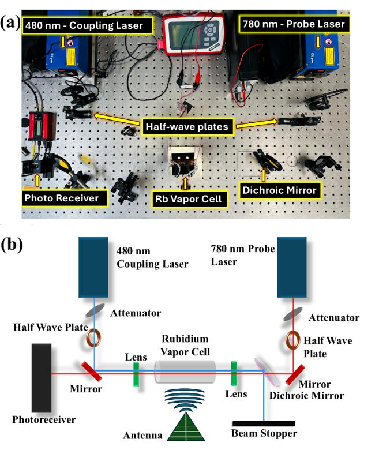
\includegraphics[width=.99\columnwidth]{F01_REAL_LAB_PHOTO.pdf}
\caption{Rydberg receiver context: (a) Experiment optical bench and (b) corresponding layout.}\label{fig:platform}
\end{figure}
\section{Background}
\subsection{From a microwave electric field to an optical observable}
In a ladder-type Rydberg-EIT measurement, a probe beam drives the rubidium ground-to-intermediate transition and a coupling beam connects the intermediate state to a Rydberg state. A microwave field couples neighbouring Rydberg levels and modifies the susceptibility experienced by the optical probe. In the appropriate near-resonant, resolved Autler--Townes limit, the RF coupling rate is
\begin{equation}
\Omega_{\rm RF}=\frac{|\boldsymbol d_{ab}\cdot\boldsymbol E_{\rm RF}|}{\hbar},
\label{eq:rabi}
\end{equation}
where $\boldsymbol d_{ab}$ is the relevant transition dipole moment. The corresponding AT separation can be related to the RF field amplitude after accounting for the atomic transition, detuning and spectral resolution\cite{Sedlacek2012,Sedlacek2013}. Figure~\ref{fig:eitphysics} illustrates the optical coupling. A true rubidium spectrum depends on Doppler averaging, optical powers and linewidths. These atomic parameters are relevant when connecting an electromagnetic simulation to a real sensor.

\begin{figure}[t]
\centering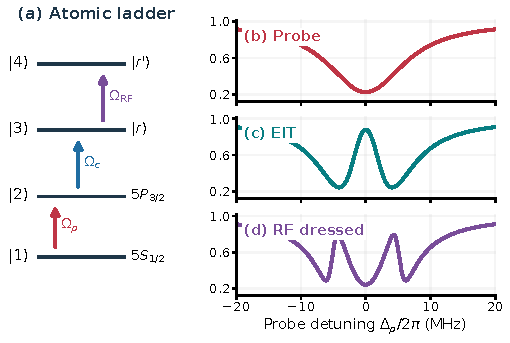
\includegraphics[width=.96\columnwidth]{F02_RYDBERG_LEVELS.pdf}
\caption{Four-level Rydberg ladder and modelled weak-probe absorption, EIT and microwave-dressed transmission.}\label{fig:eitphysics}
\end{figure}

The dot product in Eq.~\eqref{eq:rabi} explains the polarisation ambiguity. A single dipole projection constrains a field component but does not determine both transverse amplitudes and their phase. Complete transverse polarimetry instead requires independent intensity-sensitive projections that sample the Stokes information. The HFSS model constructs those projections electromagnetically; their later optical calibration remains a separate experimental task.

\subsection{Jones, Stokes and Poincar\'e representations}
Write the incident Jones vector as $\boldsymbol j=(E_x,E_y)^{\mathsf T}$ following the standard Jones/Stokes formalism \cite{Jones1941,BornWolf1999,Goldstein2011}. The Stokes four-vector $\boldsymbol S=(S_0,S_1,S_2,S_3)^{\mathsf T}$ contains total intensity, horizontal--vertical contrast, diagonal--antidiagonal contrast and circular handedness. The sign convention used throughout is $S_3=2\operatorname{Im}(E_xE_y^*)$. Purely polarised states satisfy $S_1^2+S_2^2+S_3^2=S_0^2$ and occupy the Poincar\'e sphere. The opposite circular states lie at its poles; all ideal linear states lie on the equator.

A rotated ideal linear analyser can access amplitude orientation but not circular handedness. A multi-state RF surface must therefore respond to phase quadrature as well as linear-amplitude contrast. In this study, two anisotropic copper faces and four configurable conductor gaps alter the complex transmitted Jones response. Six selected configurations are sufficient to form a full-rank Stokes observation matrix in HFSS at the reported operating points.

\subsection{Atomic receiving functional and the polarimetric gap}
The 780-nm probe interrogates the rubidium optical transition; a 480-nm coupling beam establishes a narrow Rydberg-EIT resonance, and an incident RF field mixes neighbouring Rydberg states. The photodetector measures an ensemble-averaged optical response, not the microwave field directly. Resolved AT splitting can infer the magnitude of a particular dipole projection, while finite optical linewidth, Doppler averaging and beam overlap determine how that projection is transduced into a measured spectrum. These effects belong to the subsequent optical calibration; here the electromagnetic receiver is represented by a defined quadratic field functional.

The laboratory's unsuccessful magnetic-bias discrimination scans motivated the RF-front-end approach: changing the incident microwave measurement basis offers an independent route to polarisation information without relying on small Zeeman-resolved spectral differences.

\subsection{Phase sensitivity and alternative analyser architectures}
Consider $\boldsymbol j_{\pm}=(1,\pm\mathrm i)^{\mathsf T}/\sqrt2$. Both circular states contain equal power along $x$ and $y$; they differ only in relative phase. Any device sensitive merely to $|E_x|^2$ and $|E_y|^2$ gives the same result for both. A receiver sensitive to the imaginary interference term $E_x^*E_y$, however, can distinguish their handedness. The role of the metasurface is to alter that complex receiving projection from one switch state to the next. Four independent Stokes columns make the inverse possible; singular values, absolute gain and calibration stability determine whether it is useful.

Different analysers pay for this information in different ways. Coherent vector receivers introduce RF reference fields, while spatially multiplexed metasurfaces direct polarisation components into separate output channels. Mechanical analysers rotate a receiving axis. Here a programmable RF sheet supplies sequential projections to one stationary sensing region. This avoids mechanical scanning but requires the incident polarisation to remain sufficiently stable throughout its acquisition sequence. Section~\ref{sec:em_operator} establishes the exact quadratic measurement law used to evaluate the proposed geometry.

\section{Related work and research opportunity}
\subsection{Atomic microwave field sensing}
Rydberg-based electrometry established optically interrogated RF field measurements through EIT and related spectroscopic observables\cite{Mohapatra2007,Gallagher1994,Sedlacek2012,Sedlacek2013,Holloway2014,Zhang2024,Schlossberger2024}. Contemporary atomic receivers have advanced toward frequency, phase and vector information. Three-dimensional atomic RF polarimetry has been demonstrated using orthogonal coherent reference fields\cite{Elgee2024,Cloutman2024}, while related studies have investigated polarisation-sensitive atomic mixing\cite{Yin2024}. These studies establish that atomic vector sensing is feasible. Atomic superheterodyne and phase-resolved mixing further demonstrate the importance of coherent microwave information beyond scalar splitting\cite{Jing2020,Holloway2019Mixer}. Their coherent reference architectures motivate a complementary question: can a simple passive or switchable electromagnetic front end supply several calibrated projections to a receiver with a fixed measurement axis?

The laboratory's broader research programme supplies practical context, including room-temperature broadband rubidium sensing, RF mixing studies and temperature-dependent optical receiver response\cite{Somaweera2025Review}. Those investigations place the optical receiver and its field-overlap sensitivity in context. The electromagnetic performance data analysed in the following sections come from the archived, parameterised HFSS simulations of the two-face surface.

\subsection{Polarimetric metasurfaces and microwave switching}
Instrument-matrix polarimetry is established in classical optics\cite{Azzam1988,Azzam1990,Tyo2002}. Optical metasurfaces achieve compact full-Stokes analysis through engineered anisotropy, phase-sensitive detection and spatially separated polarisation channels\cite{Arbabi2018,Basiri2019,Rubin2019,Lin2019,Ren2022,Zuo2023}. At radio and microwave frequencies, patterned conductors, frequency-selective surfaces and electronic switches provide comparable degrees of electromagnetic control, although their wavelengths and material physics differ substantially\cite{Holloway2012MS,Yu2014,Glybovski2016,Cui2014,Silaghi2021,Sofi2021,Afzal2024,Pfeiffer2013,Achouri2015}.

The closest technology comparator is electronically reconfigurable microwave polarimetry, including architectures capable of generating and detecting diverse polarisation states\cite{Chen2025Reconfigurable}. Building on this established direction, the present work develops and quantitatively optimises a compact, single-substrate, two-sided six-state analyser for a fixed receiving axis near an atomic vapour cell. The receiver-weighted spatial formulation and the matched complex-field calibration workflow define its specific contribution.

\subsection{Research opportunity}
A compact Rydberg receiver can benefit from a front end that delivers distinguishable electromagnetic responses without introducing multiple physical measurement axes into the sensing head. The research gap addressed here is an \emph{optimised RF measurement basis}: geometry should be selected to improve the rank, conditioning and usable frequency span of the resulting Stokes instrument, not only its transmission or circular dichroism. The analysis must retain the complex Jones coefficients, since amplitude-only responses cannot identify relative transverse phase.
\section{Electromagnetic modelling and verification}
\subsection{Complex-field receiving model}
\label{sec:em_operator}

Let $\boldsymbol{j}=(a,b)^{\mathsf T}$ be the incident transverse Jones vector and $\boldsymbol t_k=(t_{kx},t_{ky})$ one selected complex output row of HFSS Jones matrix $J_k$. For a specified receiving component, the state-dependent quadratic response is
\begin{equation}
 m_k=|\boldsymbol t_k\boldsymbol j|^2=\boldsymbol j^{\dagger}\mathbf H_k\boldsymbol j,
 \qquad \mathbf H_k=\boldsymbol t_k^{\dagger}\boldsymbol t_k\succeq0.
 \label{eq:main-response}
\end{equation}
With the stated harmonic convention the four incident Stokes coordinates are
\begin{equation}
\boldsymbol S=\begin{bmatrix}|a|^2+|b|^2\\|a|^2-|b|^2\\2\operatorname{Re}(a^*b)\\-2\operatorname{Im}(a^*b)\end{bmatrix}.
\label{eq:main-stokes}
\end{equation}
Writing $P_k=|t_{kx}|^2$, $Q'_k=|t_{ky}|^2$ and $C_k=t_{kx}^{*}t_{ky}$, each state yields the real Stokes row
\begin{equation}
A_k=\left[\frac{P_k+Q'_k}{2},\frac{P_k-Q'_k}{2},
 \operatorname{Re}C_k,\operatorname{Im}C_k\right].
\label{eq:main-row}
\end{equation}
Stacking the six configurations gives the physically interpretable \emph{instrument equation}
\begin{equation}
\boldsymbol m=A\boldsymbol S,\qquad
\widehat{\boldsymbol S}=A^+\boldsymbol m,
\quad A\in\mathbb R^{6\times4},\ \operatorname{rank}A=4.
\label{eq:main-inverse}
\end{equation}
For equal-power circular inputs $\boldsymbol j_\pm=(1,\pm\mathrm i)^{\mathsf T}/\sqrt 2$, the model predicts the explicit circular-response identity
\begin{equation}
 m_k(\boldsymbol j_-)-m_k(\boldsymbol j_+)=2\operatorname{Im}C_k=2A_{k3}.
 \label{eq:cp-contrast}
\end{equation}
Thus the imaginary cross-field product, not separate $|E_x|^2$ and $|E_y|^2$ magnitudes, creates handedness sensitivity. A useful analyser must retain this response across several non-coplanar Stokes rows; a large single-channel circular contrast alone is insufficient. Positive-semidefiniteness ensures $A_{k0}\ge\sqrt{A_{k1}^2+A_{k2}^2+A_{k3}^2}$. A large singular-value condition number magnifies matrix errors even if $A$ has full rank \cite{Azzam1990,Tyo2002}.


For each switch mask, two coherent orthogonal plane-wave excitations produce the complex $2\times2$ Floquet matrix $J_k(f)$. The selected output projection yields the instrument row in Eq.~\eqref{eq:main-row}. Unlike a magnitude-only transmission spectrum, the complex cross term retains the phase needed to distinguish opposite circular states. The modelled observable is electromagnetic; the optical receiver has not been assumed to measure this quadratic functional without calibration.

\subsection{Geometry parametrisation and electromagnetic optimisation}
The copper geometry uses front and rear asymmetric split-loop traces. Eleven continuous parameters describe front/rear in-plane scale, both trace widths, rear orientation, rear scale, conductor-gap length and two dimensionless gap positions. The script applies explicit width, gap and cell-clearance bounds before HFSS execution. Thirty-six candidates were evaluated using six switch states and a 41-frequency interpolating sweep from 1.0 to 2.0~GHz in 25 MHz steps. The objective favours adjacent sampled frequencies satisfying full rank, study-specific conditioning and minimum receiving-response thresholds. The reference, bandwidth-optimised and high-band alternative geometries retain an identical substrate and cell period.

\subsection{Independent-frequency and finite-array calculations}
Discovery sweeps use one frequency-adapted mesh and interpolated Jones responses; selected frequencies were subsequently resolved with independently adapted HFSS meshes. The strict dual-mesh comparison evaluates both the complex instrument and its reconstructed state transfer. We retain numerical screening thresholds of rank four, normalised condition number $\kappa_2\le35$ and a 5\% intermesh matrix agreement test, but never equate an interpolated sampled span with a guaranteed continuous bandwidth.

A separate finite-array study places nine cells on an \SI{82}{mm} square dielectric panel, with radiation boundaries and normal-incidence $x$ and $y$ illumination. The resulting total electric fields are sampled over a \SI{70}{mm}$\times$\SI{50}{mm} receiving region at planes 5, 10, 20 and 50~mm behind the surface. The finite receiver matrix is derived from these complex field maps. Field-export provenance was checked using $\boldsymbol E_{\rm total}=\boldsymbol E_{\rm incident}+\boldsymbol E_{\rm scattered}$. Mesh sensitivity is retained in the interpretation of the final results.

\subsection{Reproducible numerical procedure}
Each geometry is generated from an 11-parameter record that defines both copper faces, conductor gaps and the four ideal switch bridges. Fabrication bounds are applied before meshing; invalid polygons are rejected. Six masks are simulated under the same unit-cell pitch and substrate assumptions. For every mask, the two incident polarisation bases yield complex transmitted coefficients, preserved with their port and time-harmonic conventions. This is essential: changing the reference direction or handedness convention can reverse $S_3$ while leaving magnitude-only $S$-parameter plots apparently unchanged.

The study has two numerical stages. The 25-MHz discovery grid identifies candidate frequency intervals using interpolated sweeps; selected frequencies are then rerun with independent adaptive meshes to test complex-instrument agreement. Failed or incomplete convergence gates remain part of the record. The finite $3\times3$ calculation is treated separately: it uses total fields, checked against incident-plus-scattered exports, and integrates their coherent two-basis combinations over the stated receiving region. Native copper polygons, complex Jones coefficients, switch masks, solver status and the resulting instrument matrices are retained so the principal plots can be regenerated without digitising images.

\subsection{HFSS solution setup and quality assurance}
A repeatable microwave simulation must specify both what it solves and what it extracts. For the periodic structure the Floquet ports excite two orthogonal transverse polarisations while master/slave or the equivalent periodic constraints model a repeating unit cell. The physical material stack consists of a dielectric sheet with patterned conductors on opposing faces. The geometry is normalised to a 24-mm cell and the relative phase between the two incident basis excitations is preserved. The complex transmitted modal coefficients are read from the same port convention for all six switching states and frequencies. This matters because a sign inversion, port-direction reversal or swapped linear basis can change inferred Stokes handedness without making a magnitude-only S-parameter spectrum look suspicious.

A separate empty-cell or empty-board reference provides a consistent electromagnetic baseline. It is not a substitute for an independent measurement axis: it corrects or documents common propagation and substrate effects while the switched states supply the polarimetric diversity. The instrument rows are derived from the complex Jones matrices, and calibration data are retained with their HFSS setup identifiers. The optimisation compares candidate structures at equal unit-cell pitch and material-stack assumptions; otherwise the apparent gain of a geometry change could be caused by a different aperture or reference setup.

The selected-frequency verification is intentionally more expensive than the discovery sweep. A discrete adapted HFSS solution examines the response at one particular frequency with its own local mesh; two such solutions, using controlled refinement policies, allow the complex Jones coefficient vector to be compared. A small difference between the resulting instrument matrices supports numerical repeatability. A different criterion evaluates what happens if an instrument calculated from one mesh is used to invert observations generated by another. These two tests answer different questions: matrix change measures electromagnetic coefficient stability, whereas cross-model inversion assesses how that change is amplified by the inverse operator. The latter is particularly sensitive when a measurement basis is nearly singular.

The FEM meshes are not calibrated physical measurements; they are numerical approximations that become more useful when the relevant outputs stabilise under independent refinement. Earlier simulations in this project sometimes reached the maximum adaptive passes without meeting their actual convergence targets. The later campaigns therefore captured HFSS native convergence files and compared both the declared setting and the criterion actually used by the solver. For the finite plane-wave problem, the relevant adaptive criterion was the magnetic-energy change rather than the port-based Delta-S quantity. The distinction explains why a solver can report completion while local near-field predictions remain insufficiently converged for a numerical accuracy claim.

Available computational resources imposed a practical ceiling on the most aggressive finite-array mesh refinements. This is not a physical limitation of the proposed surface. Accordingly, the thesis distinguishes a completed finite-field data set from a fully mesh-independent field solution. The former is still scientifically useful because it demonstrates full-rank behaviour and clear observation-plane dependence; the latter remains a defined target for a follow-on refinement campaign.

\subsection{Instrument construction and physicality checks}
For a complex Jones row $\boldsymbol t_k=(t_{kx},t_{ky})$ representing a selected receiving axis, define the non-negative Hermitian matrix $\mathbf H_k=\boldsymbol t_k^{\dagger}\boldsymbol t_k$. The expected quadratic output is $m_k=\boldsymbol j^{\dagger}\mathbf H_k\boldsymbol j$. Since $\mathbf H_k$ is positive semidefinite, its eigenvalues cannot be negative. This basic constraint is a useful implementation check: a fitted analyser row that predicts negative power for a physically admissible Stokes vector is inconsistent with the specified receiving model or has been processed with incompatible conventions.

Each Hermitian $2\times2$ response can be represented by a four-element real Stokes measurement row. The full instrument $A\in\mathbb R^{6\times4}$ therefore maps the four incident Stokes coordinates into six real model observations. A rank-four instrument admits a least-squares inverse even though it contains redundant measurements. If the rows are too similar, the smallest singular value becomes small and the inverse is poorly conditioned. The numerical pipeline reports all four singular values and the normalized condition number, since rank alone is an inadequate measure of polarisation discrimination quality. The six measurements also provide an opportunity to check internal consistency of the linear model because the observed response vector occupies the column space of $A$ in the ideal calculation.

The full derivation in Appendix~\ref{sec:derived} generalises the operator from a single projected Floquet coefficient to a spatially weighted receiving region. That generalisation is central to the finite HFSS study: different incident polarisations produce different complex total-field distributions, and the receiver effectively weights the two orthogonal basis fields according to its position and extent. An intensity-like integration over a specified region yields a physically non-negative quadratic form and an explicit measurement row. Changing that region changes the actual measurement definition. The board and the atomic optical mode consequently need to be optimised together in any future complete receiver design.

\section{Measured linear-polarisation response}
\begin{figure}[tb]
\centering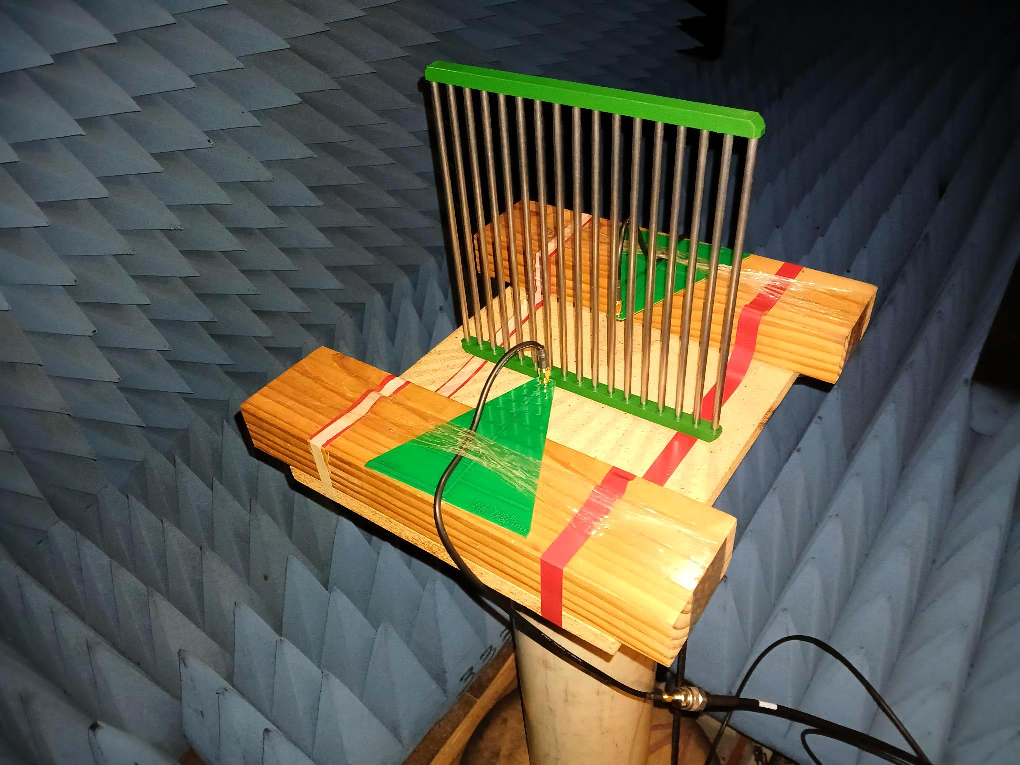
\includegraphics[width=.98\columnwidth]{F06_PHOTOGRAPHIC_POLARISER.pdf}
\caption{Measured linear-polariser fixture used for the orientation-discrimination campaign.}\label{fig:linearphotos}
\end{figure}
\subsection{Theory and experimental method}
An ideal linear analyser transmits the electric-field component aligned with its axis. For incident linear polarisation at relative angle $\theta$, the familiar intensity law is $I(\theta)\propto\cos^2\theta$; real RF polarisers exhibit finite extinction, insertion loss and geometry-dependent departures from this reference. The laboratory campaign used a linear source, a metal-rod polarising structure and a receiving arrangement near 2~GHz to quantify orientation-dependent attenuation. A separate interim VNA campaign characterised the steel-rod polariser and the magnetic-bias coil. These are different source datasets and are reported as such.

\subsection{Measured results}
The later archived point readings were $-8.2$~dBm without the front-end polariser, $-13.9$~dBm in the preferred orientation, $-15.1$~dBm at nominal $45^\circ$ and $-23.6$~dBm in the rejected orientation. The preferred-to-rejected contrast is \textbf{9.7~dB}. The independent June laboratory measurement record recorded approximately 14--15~dB pass/reject VNA contrast for the custom steel-rod configuration. Figure~\ref{fig:linearresults} displays the original archived point values directly without interpolated measurements or a fitted angle curve. The experimental trend is consistent with substantial linear-orientation selectivity.

\begin{figure}[t]
\centering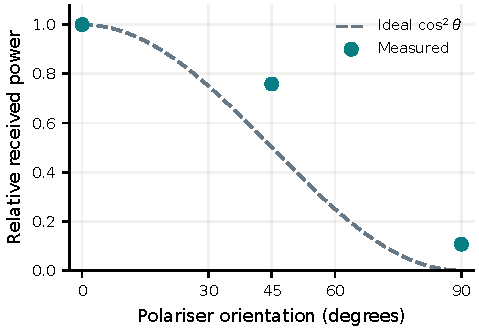
\includegraphics[width=.99\columnwidth]{FINAL_F06_LINEAR_EXPERIMENT.pdf}
\caption{Linear-polariser measurements and the ideal $\cos^2\theta$ reference (guide only; not a fitted response).}\label{fig:linearresults}
\end{figure}

The reported preliminary normalised equatorial Stokes estimate was $s_1\simeq0.806$, $s_2\simeq0.370$. Its projected azimuth is $\tfrac12\mathrm{atan2}(s_2,s_1)\simeq12.3^\circ$; this estimate contains no independently recovered circular coordinate $s_3$. The measurement therefore motivates a state-dependent RF analyser that adds a phase-sensitive response while keeping the existing Rydberg platform conceptually simple. The coil calibration $B_0(I)\simeq2.302I+0.028$~mT and its reported $R^2=0.981$ document an additional experimental subsystem; they are not used to manufacture a polarisation result.

\subsection{Experimental interpretation and measurement limits}
The four later received-power readings support two meaningful performance quantities. The 9.7-dB preferred-to-rejected difference quantifies angular discrimination between two configurations of the measured polariser. By contrast, the difference of 5.7~dB between the unscreened path and the preferred orientation includes the presence of the structure and the changed test path. It would therefore be misleading to call both numbers extinction ratio. The raw dBm difference between preferred and rejected positions corresponds to a received-power ratio of approximately $10^{9.7/10}\approx9.33$, under the usual matched-power interpretation. The ratio gives a useful sense of orientation selectivity without imposing an optical Malus-law fit on four heterogeneous RF point measurements.

The earlier steel-rod VNA campaign and later orientation-dependent receiving experiment should not be merged into one fitted series. Different antennas, references, sample geometry and receiver channels can shift absolute received power and apparent contrast. The reported 14-15-dB interim result is valuable independent validation that the hardware architecture could substantially discriminate orientation, whereas the later 9.7-dB result illustrates its response in the context of a different readout chain. Both can be included in a final engineering account when their apparatus and definitions are specified separately.

The reported partial linear Stokes values also have a precise limit of interpretation. An observed $(s_1,s_2)$ point estimates a projection onto the equatorial plane but does not determine $s_3$. Many elliptic states share the same linear coordinates while differing in handedness content. The experiment therefore supplies a clear motivation for the phase-sensitive metasurface: it provides the missing physical category of measurement without requiring the experimental record to imply a full polarisation measurement that was not performed.

\section{Reconfigurable two-face metasurface: design theory}
\subsection{Why two anisotropic layers are useful}
A useful circular analyser must discriminate fields of equal transverse intensity but opposite relative phase. A single real-valued projection provides linear-amplitude discrimination, whereas coupling between differently oriented resonant currents can generate the complex off-diagonal Jones coefficients needed to weight $S_3$. In a compact printed surface, trace length contributes inductive loading, open gaps contribute capacitive loading and the two opposed copper faces couple electromagnetically through the substrate. Changing the conduction across selected gaps alters these interactions and consequently changes the Stokes analyser row.

The implemented geometry uses a split-loop-like copper path on each face of one dielectric sheet. The rear path is mirrored, rotated and scaled relative to the front. Four ideal conductor-switch sites are distributed across both faces, and six switch combinations were selected for numerical inversion. Figure~\ref{fig:layout} places three complementary views side by side: the simulated $3\times3$ array, the native HFSS unit cell and a reduced-order modal analogue. The four D1--D4 markers indicate the actual geometric bridge locations in the archived simulation, with D1--D2 on the front conductor path and D3--D4 on the rear path. Panel~(c) interprets the structure as two coupled resonant current modes linked by electric and magnetic coupling, while each geometric interruption is represented by a gap capacitance that can be bypassed by a PIN-diode bridge. The analogue is physically motivated rather than parameter-extracted: it is intended to explain how switching selected gaps perturbs the resonance and cross-coupling pathways that determine the analyser row.

\begin{figure*}[t]
\centering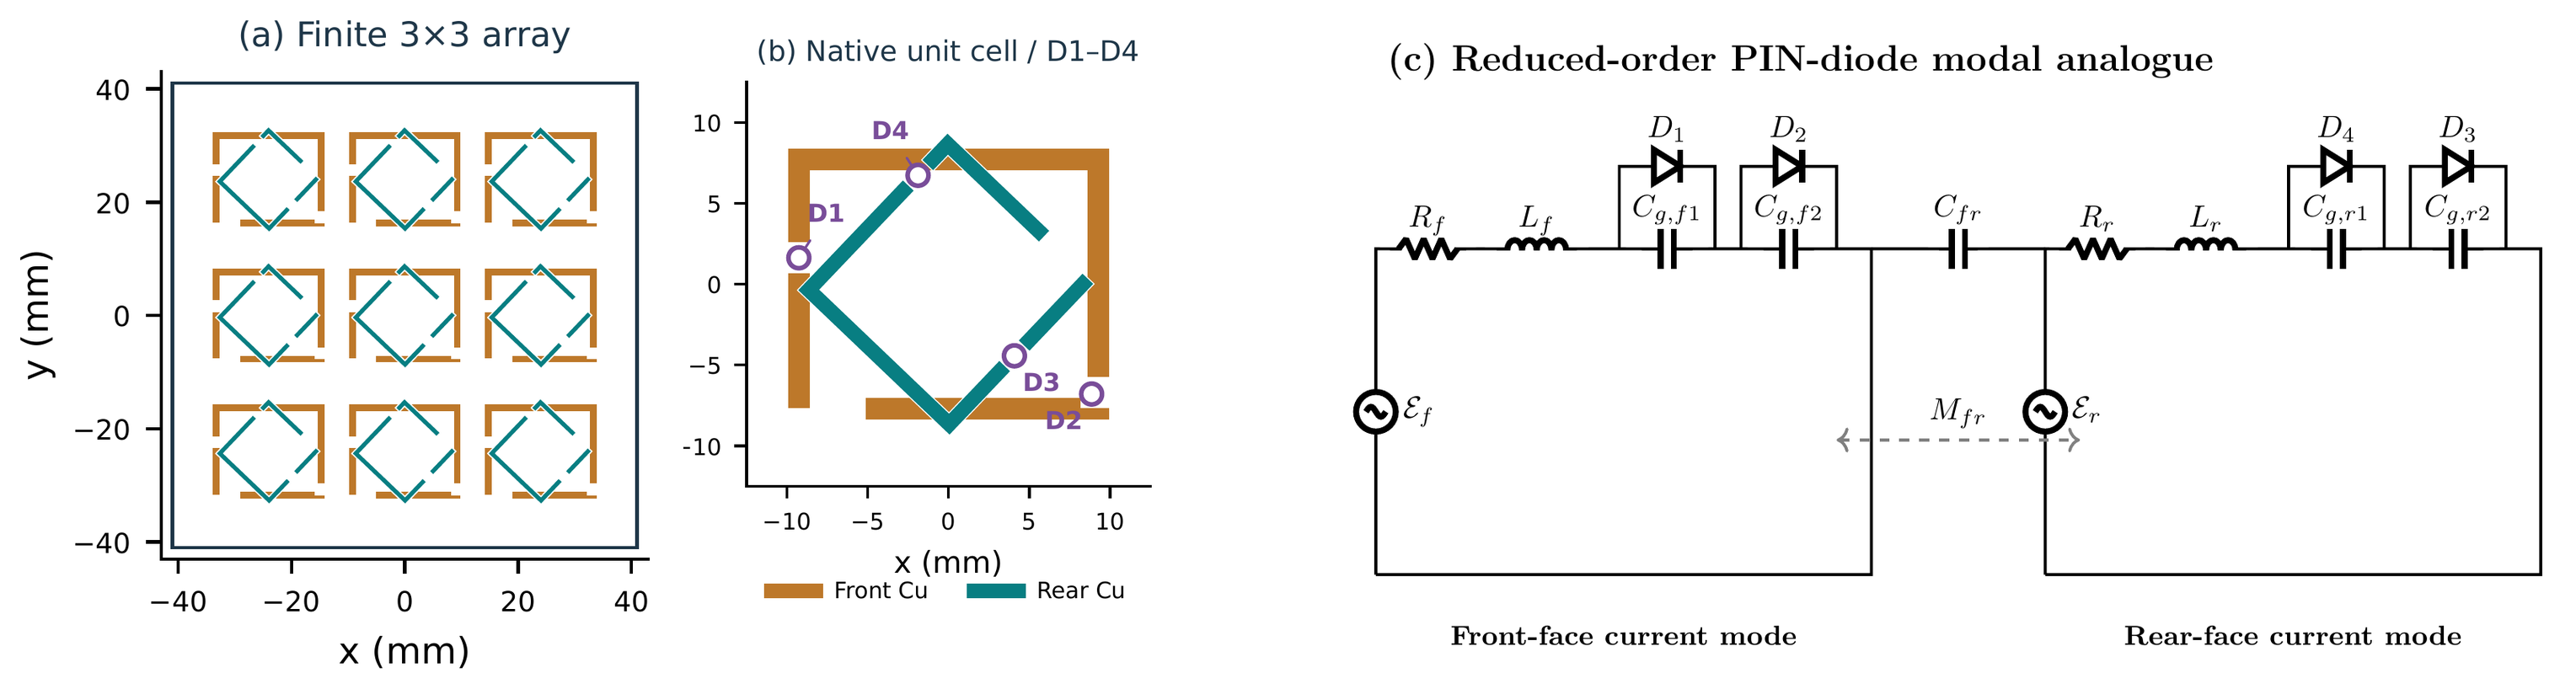
\includegraphics[width=.995\textwidth]{FINAL_F04_FINITE_PCB_METATOM_CIRCUIT.png}
\caption{C033 architecture presented in three side-by-side views. (a) Finite $3\times3$ panel. (b) Native copper geometry and bridge sites D1--D4, where D1--D2 interrupt the front conductor path and D3--D4 interrupt the rear path. (c) Reduced-order PIN-diode modal analogue showing front-face and rear-face resonant current loops, gap capacitances, diode-bypass branches and interlayer electric ($C_{fr}$) and magnetic ($M_{fr}$) coupling. The circuit is an interpretive model; its element values were not extracted from HFSS.}\label{fig:layout}
\end{figure*}

\begin{figure}[tb]
\centering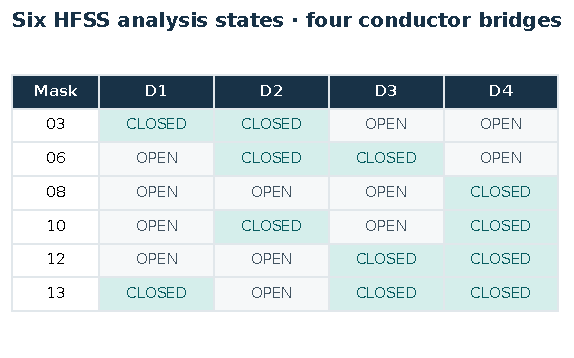
\includegraphics[width=\columnwidth]{F05_SWITCHING_COMPACT.pdf}
\caption{Six programmed conducting-bridge masks used for Stokes analysis.}\label{fig:switchmap}
\end{figure}

\subsection{Polarisation measurement rather than polarisation generation}
The design objective is measurement-state diversity. It is not necessary that every switched structure emit an arbitrary target polarisation. Instead, its response to a fixed unknown incident field must provide an independent row of the common Stokes observation matrix. The tensor quantities responsible for coupling and circular sensitivity arise from the \emph{complex} Jones response; consequently, simulated reflection or transmission magnitudes alone are insufficient for full-Stokes analysis. This distinction motivates the project-derived receiving operator, rank test and numerical condition-number objective.

\subsection{Equivalent-circuit interpretation and switching-state diversity}
The conductor path and interruption points can be interpreted through the stored-field physics of distributed microwave networks. Current along the elongated copper traces produces magnetic energy and an effective series inductive loading. Open gaps between conductor ends support local electric fields and capacitive displacement currents. Placing two different traces on opposite faces of a dielectric adds interlayer electric and magnetic coupling, including a phase delay associated with the geometry. The resulting array is not simply a conventional lumped $L$--$C$ filter; rather, the equivalent elements explain why a changed physical conducting path can shift resonance, transmission phase and cross-polarisation conversion. Numerical element values would require a dedicated full-wave network extraction; none are assigned here.

Each proposed PIN-diode position is a switch site between two conductor sections. The ideal HFSS model represents a closed state as an inserted conducting bridge and an open state as a gap. This construction is a controlled initial step because it isolates the influence of topology before manufacturer-specific diode parasitics and DC-bias traces are selected. A physical PIN implementation would require an ON-state series resistance and package inductance, an OFF-state junction capacitance, RF chokes or bias tees where appropriate and a bias-routing topology that does not spoil the desired current distributions. Figure~\ref{fig:layout}(c) makes this interpretation explicit. The voltage sources represent the incident field's effective electromotive drives, not external laboratory generators. Each labelled break in panel (c) corresponds to a geometric interruption in panel (b): D1 and D2 bypass the front-face gap capacitances, while D3 and D4 bypass the rear-face gap capacitances. The coupling terms $M_{fr}$ and $C_{fr}$ represent, respectively, magnetic and electric interaction between the two modal current paths. The drawing is therefore a reduced-order explanatory network that preserves the physical role of the four diode sites while avoiding the false precision of an unfitted extracted circuit.

There are sixteen possible four-bit conductor states in principle. This work selects six masks that exhibit useful and distinct Jones projections. The state choice is a polarimetric measurement-basis decision rather than a digital modulation alphabet. The array is interrogated sequentially under the assumption that incident polarisation is stationary over an acquisition sequence, or that its evolution can be tracked by a sufficiently rapid controller. The important calibration output is therefore a row of the Stokes instrument for each selection. Equal transmitted power under one incident input does not imply equal utility: two states can respond almost identically to horizontal radiation yet differ markedly when the input includes circular quadrature.

The geometric constraints also govern the physical plausibility of the proposed PCB. The copper exists on two accessible external faces of a single dielectric sheet, and the high-level model uses a 1.6-mm board thickness. The chosen front and rear trace widths lie comfortably above the project's nominal minimum-feature target. Nonetheless, optical access through the full vapour-cell region, the substrate's frequency-dependent permittivity, copper plating, bias routing, drill/via requirements and diode footprint cannot be inferred from ideal-PEC field plots. The numerical model demonstrates an electromagnetic concept with parameter bounds; it is not a signed-off PCBWay fabrication package.


\subsection{Reduced coupled-resonator response and circuit interpretation}
The two patterned conductors represented by the equivalent circuit in Fig.~\ref{fig:layout}(c) admit a reduced-order, frequency-dependent description based on their distributed magnetic and electric stored energies. For $q\in\{f,r\}$ denoting the front or rear copper face, define the gap impedance for switching state $s$ by
\begin{align}
 Z_{g,q}(\omega,s)&=\big[j\omega C_{g,q}+Y_{D,q}(\omega,s)\big]^{-1},\notag\\
 Z_q(\omega,s)&=R_q+j\omega L_q+Z_{g,q}(\omega,s).
 \label{eq:circuit_gap}
\end{align}
An ideal open conductor bridge has $Y_{D,q}=0$, while an ideal closed bridge has $Z_{g,q}\rightarrow0$. A packaged PIN diode can be represented, after physical selection and extraction, by an ON-state $R_{\mathrm{on}}+j\omega L_{\mathrm{pkg}}$ branch or an OFF-state junction capacitance and leakage conductance. The four HFSS bridge locations interrupt different current paths. Accordingly, $Y_{D,q}$ in Eq.~\eqref{eq:circuit_gap} is a representative modal admittance, not a netlist of the four PIN-diode devices. The physical bridge connectivity is defined by panel (b), while the reduced network explains the first-order field mechanism.

A first-order coupled-mode circuit for the two resonant traces is
\begin{equation}
\begin{pmatrix}Z_f&j\omega M_{fr}\\j\omega M_{fr}&Z_r\end{pmatrix}
\begin{pmatrix}I_f\\I_r\end{pmatrix}
=\begin{pmatrix}V_f^{\mathrm{inc}}\\V_r^{\mathrm{inc}}\end{pmatrix},
\label{eq:coupled_circuit}
\end{equation}
with additional displacement-current coupling represented by $C_{fr}$ in the nodal network. The drives $V_{f/r}^{\rm inc}$ depend on the incident Jones vector and conductor orientation. The interference of the resulting complex currents changes the anisotropic Jones transmission tensor; it is the \emph{imaginary} field-overlap term, rather than extinction alone, that gives the reconstructed instrument sensitivity to $S_3$. A quantitative circuit model would require fitting the complex scattering response and checking reciprocity and passivity; the present diagram is restricted to explaining the physical coupling mechanism.

A practical design condition follows by considering the matrix-resolvent sensitivity $\partial \mathbf{Z}^{-1}/\partial p=-\mathbf{Z}^{-1}(\partial \mathbf Z/\partial p)\mathbf{Z}^{-1}$. Geometry parameters or bridge states that strongly perturb the coupled-impedance matrix can rotate the complex receiving vectors; the optimisation seeks \emph{diversity} of those vectors rather than merely maximising a single transmission coefficient. This gives a direct circuit-level rationale for simultaneously screening state gain, circular response and instrument conditioning.

\subsection{How the geometry parameters affect the measured response}
The front and rear conductor shapes are deliberately related but not identical. Separate $x$ and $y$ scale parameters determine their projected lengths and the relative detuning of the orthogonal current paths. Trace widths influence the distributed inductance, conductor current distribution and gap-field concentration. The rear-layer rotation changes how the two anisotropic paths couple under incident fields aligned with the laboratory axes. The additional rear scale parameter adjusts their relative size, while the gap locations determine which portions of the resonant paths are interrupted when a switch opens. Altering a gap position may change the polarisation response even when the total copper area changes only slightly, because it moves the discontinuity relative to current antinodes and phase-sensitive coupling regions.

The parameters were varied within bounded ranges to preserve the nominal unit-cell footprint and conductor dimensions. The resulting optimization is not a search among completely unrelated shapes; it is a systematic experiment inside a controlled family of two-face split loops. This matters when interpreting the chosen design. The improved condition and sampled operating span can be attributed to changed geometrical relationships within one architecture, not to an uncontrolled change from one kind of antenna or substrate to another. At the same time, the limited search family places an honest boundary on the word \emph{optimal}: the reported candidates are the best found among the evaluated parameter combinations and their stated screening objective, rather than a proof of globally optimal full-Stokes measurement.

The comparison can be understood in terms of an instrument basis on the Poincar\'e sphere. An idealised highly symmetric set of measurement projections is distributed so that no Stokes coordinate is observed much more weakly than the others. The present planar geometry cannot directly impose those ideal points at will; instead, HFSS supplies a physically constrained set of analyser rows for each switch pattern. Optimising geometric dimensions changes both the length and direction of those rows in Stokes space. The condition number measures the spread of these independent response directions after gain normalisation: a value of 9.53 indicates a substantially less ill-conditioned inversion than 34.62, but neither value is a percentage error nor a noise-independent accuracy guarantee. The minimum response metric separately guards against a well-conditioned matrix built from nearly undetectable signals. This joint optimisation gives the final design a more meaningful interpretation than a narrow resonance tune.

\section{Geometry optimisation and full-Stokes simulation results}
\subsection{Optimisation history and candidate selection}
The reference design passes eight adjacent frequencies on the original 25-MHz discovery grid, spanning 1.825--2.000~GHz (175-MHz endpoint difference). Both optimised designs pass eleven sampled points, yielding a 250-MHz endpoint difference. The 42.9\% span increase is a \emph{sampled HFSS discovery metric}, established across 36 actual candidate HFSS campaigns. It does not prove that every frequency between the sampled endpoints or any untested frequency beyond 2~GHz satisfies the full-Stokes criterion. Figure~\ref{fig:optresults} shows the complete candidate ranking and the trade-off between sampled span and matrix conditioning.

\begin{figure*}[t]
\centering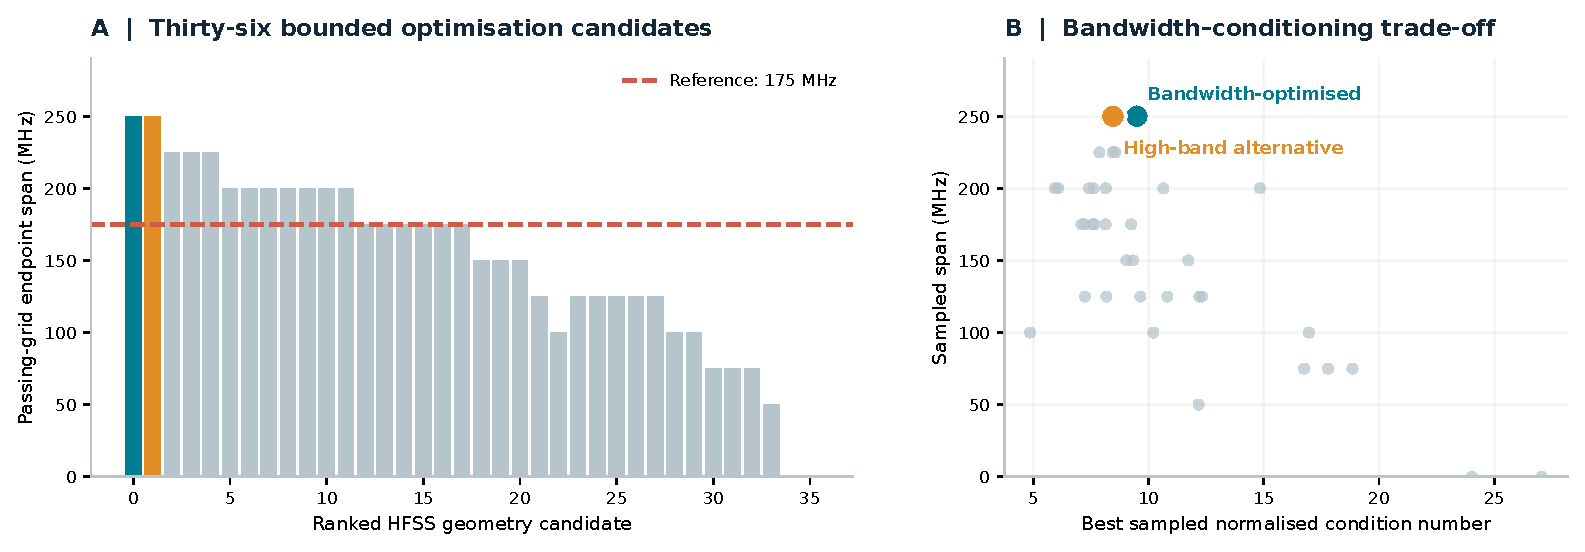
\includegraphics[width=.98\textwidth]{FINAL_F07_OPTIMISATION.pdf}
\caption{HFSS search across 36 candidate geometries; dashed line marks the 175-MHz reference screening span.}\label{fig:optresults}
\end{figure*}


\subsection{Optimisation metrics and what their improvement means}
The optimisation objective is based on the receiving matrix rather than on an isolated S-parameter peak. First, an instrument must be rank four: the selected RF transformations cannot all project onto one linear subspace. Second, the rows must possess sufficient directional diversity, assessed through the condition number after row normalization. Third, the response should not vanish in one state, because a mathematically independent but arbitrarily weak measurement channel would be difficult to calibrate. A useful frequency requires all these criteria to be considered together. The screening thresholds are engineering decisions declared before evaluation, not universal definitions of a polarimeter's usable bandwidth.

The discovery score counts adjacent passing samples on a 25-MHz grid. Eleven points rather than eight give a 250-MHz rather than 175-MHz endpoint span, a 42.9\% improvement in this \emph{screening measure}. The complete 36-candidate ranking is retained in Fig.~\ref{fig:optresults}, which shows the distribution of outcomes rather than only the best geometry. Because a narrow untested resonance could occur between adjacent grid points, the resulting interval is not claimed as a continuously verified operating band. The independent adaptations below test individual frequencies more rigorously.

\subsection{Independent-frequency HFSS verification}
\label{sec:conditioningexplained}

\noindent\textbf{How to interpret a condition number.} The six HFSS responses produce a $6\times4$ matrix $A$ that maps four incident Stokes parameters into six simulated observations. Rank four establishes that the four unknowns can be distinguished in an ideal noiseless calculation; it does \emph{not} establish that the inverse is insensitive to errors. Let $\widetilde A=D^{-1}A$, where the diagonal matrix $D$ contains the positive reference gain of each state. The spectral condition number is
\begin{equation}
\kappa_2(\widetilde A)=\frac{\sigma_{\max}(\widetilde A)}{\sigma_{\min}(\widetilde A)},
\label{eq:condition_interpretation}
\end{equation}
where $\sigma_{\max}$ and $\sigma_{\min}$ are the largest and smallest singular values. A value closer to one means the polarisation directions are interrogated more evenly. A larger value means that perturbations along a weakly observed direction may be amplified more severely. For a fixed matrix, normalised observations $\widetilde{\boldsymbol m}=\widetilde A\boldsymbol S$ and a consistent perturbation obey the conservative bound
\begin{equation}
\frac{\|\delta\boldsymbol S\|_2}{\|\boldsymbol S\|_2}
\le \kappa_2(\widetilde A)
\frac{\|\delta\widetilde{\boldsymbol m}\|_2}
{\|\widetilde{\boldsymbol m}\|_2}.
\label{eq:condition_error_bound}
\end{equation}
For example, $\kappa_2=9.53$ means that a 1\% relative perturbation in the \emph{consistently normalised} observations gives a worst-case bound of about 9.53\% relative reconstruction error under this model. It does \emph{not} predict a typical 9.53\% error and does not include uncertainty in the calibration matrix. The value 35 was the project's \emph{screening threshold}, not a universal benchmark for polarimeter accuracy.

A separate dual-mesh campaign independently adapted the six state-dependent HFSS solutions at selected frequencies. The bandwidth-optimised design retained full rank and reached normalised condition number 34.62 at 1.750~GHz, 9.53 at 1.925~GHz and 16.84 at 1.975~GHz. At 1.925~GHz its relative Stokes instrument-matrix change between mesh levels was 0.551\%, while the deterministic calibration-transfer discrepancy on the defined numerical test set was 5.01\%. The high-band alternative yielded a condition number of 8.64 at 1.950~GHz with 0.325\% matrix change. These selected-frequency results provide stronger evidence than the discovery interpolation alone.

The smaller value at 1.925~GHz means that a specified relative error in \emph{normalised} observations has a substantially smaller worst-case amplification bound than at 1.750~GHz. In physical terms, the six switch states provide more independent views of polarisation at this frequency. However, the condition number alone does not establish detector signal-to-noise ratio, because row normalisation removes absolute-gain differences. It must be read alongside the gain-aware and mesh-transfer results that follow. In particular, 0.551\% agreement between the two periodic HFSS matrices describes the \emph{forward model}; the separately computed 5.01\% calibration-transfer discrepancy shows why it must not be reported as a 0.551\% Stokes reconstruction error.

\begin{figure*}[t]
\centering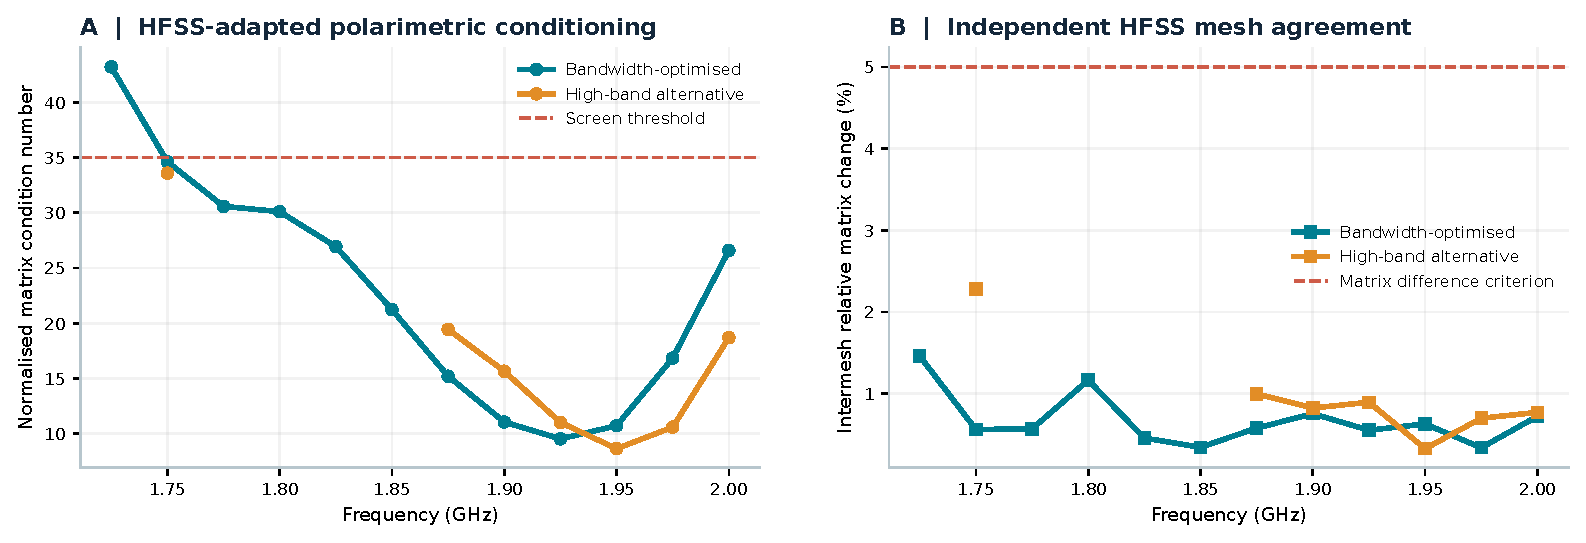
\includegraphics[width=.96\textwidth]{FINAL_F08_ADAPTED_RESULTS.pdf}
\caption{Independently adapted HFSS frequencies: polarimetric condition number and matrix agreement for the optimised candidates.}\label{fig:adapted}
\end{figure*}

The reference design separately achieved a rank-four matrix at 1.850~GHz with normalised condition number 22.06 and 0.749\% intermesh matrix difference. Its controlled-mesh response provides a stable baseline against which optimisation was evaluated. Because lower condition numbers at very different frequencies cannot be compared as an isolated performance improvement, the figure preserves frequency on the horizontal axis for both candidates.

\subsection{Algebraic Stokes observability}
The six programmed periodic Jones responses form a rank-four instrument at the selected operating frequency. For a prescribed Stokes vector, its quadratic model and Moore--Penrose inverse satisfy $A^{+}A\boldsymbol S=\boldsymbol S$ when $A$ has full column rank. This self-inversion verifies the computational convention rather than predicting fabrication accuracy. An independent-mesh finite-panel reconstruction study is retained in Appendix~\ref{app:finite}; its outcome is not used to overstate the periodic surface's demonstrated performance.


\subsection{Polarisation information carried by the six switch states}
A full-rank instrument need not require every programmable state to contribute equally. This matters in hardware: unnecessary switching adds acquisition time, whereas omitting an informative state can amplify calibration and readout errors. We therefore use the independently adapted C033 Jones responses at 1.925 GHz to study the information geometry of the \emph{actual} six-state design, rather than assigning all states equal engineering value by assumption.

Let $A\in\mathbb R^{6\times4}$ be the HFSS-derived quadratic instrument and let $P=\operatorname{diag}(A_{10},\ldots,A_{60})^{-1}A$ denote its row-gain-normalised form. For an incident Stokes vector $S$ with $S_0=1$, the normalised response to mask $k$ is
\begin{equation}
 y_k=\frac{m_k}{A_{k0}}=P_{k:}S,\qquad
 P_{k:}=\left(1,\mathbf p_k^{\mathsf T}\right).
 \label{eq:v41_norm_response}
\end{equation}
In Fig.~\ref{fig:v41_response}(a), the columns correspond to the horizontal, vertical, diagonal, antidiagonal and two opposite circular Stokes basis states. Each displayed number is a response computed from the archived complex HFSS coefficients, not an independent microwave or optical measurement. In particular, $y_{k,R}-y_{k,L}=2P_{k3}$ explicitly identifies which states discriminate circular handedness. The response diversity confirms rank four, but the unevenness of the rows motivates a state-selection study.

\begin{figure*}[t]
\centering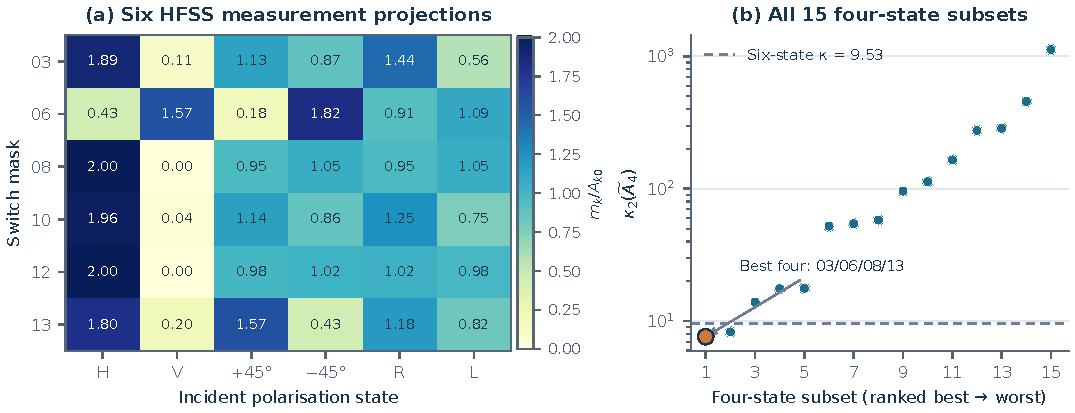
\includegraphics[width=.91\textwidth]{V41_FIG_RESPONSE_AND_SUBSETS.pdf}
\caption{HFSS-derived polarisation response and all 15 four-state sub-instruments at 1.925 GHz. The heat map shows normalised predicted quadratic observations for six fully polarised Jones inputs; the right panel compares conditioning of every four-state choice with the complete six-state matrix.}\label{fig:v41_response}
\end{figure*}

\subsection{A state-selection law: observability versus stability}
A four-state analyser is algebraically sufficient because the unknown Stokes vector has four components, but in practice the determinant, singular spectrum and receiving gain determine whether those four equations can be trusted. Every additional state requires another stationary-field acquisition, so acquisition time and uncertainty must be considered together. The exhaustive $\binom64=15$ search below tests every four-state subset of the existing six-mask design; it does not invent a seventh or eighth electromagnetic state. In a future physical receiver, the switching period must also be short compared with the coherence time of the incident polarisation.


To turn the above picture into a reproducible engineering decision, consider equal-variance perturbations to the *normalised* scalar outputs; this is a design comparator, not an assertion about measured detector noise. Define the information matrix $F=P^{\mathsf T}P$ and its inverse-trace diagnostic $J=\operatorname{tr}(F^{-1})$. Then the linear least-squares covariance is $\sigma^2F^{-1}$ if the six normalised readouts have independent common variance $\sigma^2$. For the independently adapted C033 periodic matrix at 1.925 GHz we obtain
\begin{equation}
 \operatorname{rank}P=4,\quad \kappa_2(P)=9.5282,\quad
 \operatorname{tr}[(P^{\mathsf T}P)^{-1}]=13.9407.
 \label{eq:v41_result}
\end{equation}
Enumerating all $\binom64=15$ four-state choices yields a \emph{best subset by condition} with masks 03, 06, 08 and 13: its condition number is 7.63, but its inverse-trace diagnostic increases to 16.02. Thus a numerically smaller condition number does not imply better total least-squares precision; the additional states improve total information while sometimes increasing the ratio between extreme singular values. At the other extreme, poorly chosen four-state subsets have conditions above $10^3$ despite still being algebraically full rank.

The importance of a particular state follows from an exact rank-one identity. With row $\mathbf p_k^{\mathsf T}=P_{k:}$ and leverage $h_k=\mathbf p_k^{\mathsf T}F^{-1}\mathbf p_k$, omitting that observation gives $F_{-k}=F-\mathbf p_k\mathbf p_k^{\mathsf T}$. Provided $h_k<1$ and the reduced matrix remains nonsingular, the Sherman--Morrison identity yields
\begin{equation}
 F_{-k}^{-1}=F^{-1}+\frac{F^{-1}\mathbf p_k\mathbf p_k^{\mathsf T}F^{-1}}{1-h_k}.
 \label{eq:v41_state_drop}
\end{equation}
The second term is positive semidefinite. It proves that adding a calibrated observation cannot worsen the inverse-trace criterion under this equal-variance model, even though its *condition number* need not improve. Figure~\ref{fig:v41_leverage} applies Eq.~\eqref{eq:v41_state_drop} directly to the C033 matrix. Omitting mask 06 increases $J$ by a factor of 86.4, and omitting mask 13 increases it by 35.6; the remaining masks have smaller effects. Masks 06 and 13 are therefore disproportionately important in the normalised geometry. There is a practical counterweight: mask 06 also has the smallest raw scalar gain, $A_{20}=0.0550$, compared with 0.336--0.451 for several other states. Equal variance *after* normalisation is not guaranteed by an RF power detector. A physical noise or calibration model should consequently use the unnormalised operator $A$ and a measurement covariance $\Sigma_m$, with information $A^{\mathsf T}\Sigma_m^{-1}A$. For the stored C033 matrix the raw condition is 18.48, versus 9.53 after gain normalisation. This trade-off suggests an explicit engineering priority: preserve the basis diversity supplied by masks 06 and 13 while improving the received gain and repeatability of the weak-gain state.

\begin{figure}[t]
\centering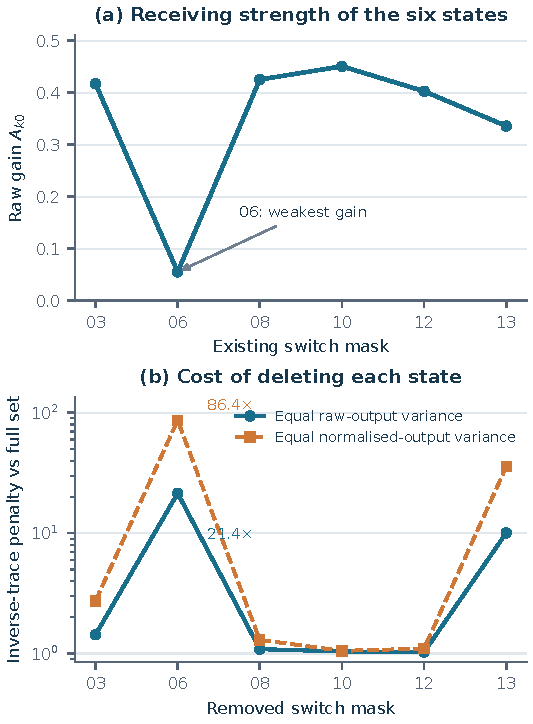
\includegraphics[width=.98\columnwidth]{V51_FIG_GAIN_AWARE_INFORMATION.pdf}
\caption{Gain-aware C033 state analysis, shown as vertically stacked single-column subplots: (a) absolute HFSS row gain and (b) inverse-trace penalty under different equal-variance assumptions.}\label{fig:v41_leverage}
\end{figure}

\subsection{A gain-aware law for state selection}
The preceding state-selection test exposes a subtle engineering hazard: row-gain normalisation makes the Stokes directions comparable, but it also suppresses differences in received signal strength. A weak state can appear indispensable under an assumed equal variance for all \emph{normalised} measurements, even though this is not the noise model of a detector whose additive uncertainty is approximately constant before normalisation. The appropriate information matrix for a calibrated six-state model is
\begin{equation}
\mathcal I(\boldsymbol A,\boldsymbol\Sigma)=\boldsymbol A^{\mathsf T}\boldsymbol\Sigma^{-1}\boldsymbol A,
\qquad \operatorname{Cov}(\widehat{\boldsymbol S})=\mathcal I^{-1},
\label{eq:v42_information}
\end{equation}
where the covariance equality applies to a full-rank linear model with independent unbiased errors and known positive-definite covariance $\boldsymbol\Sigma$. With $g_k=A_{k0}>0$ and $\widetilde{\boldsymbol A}=\boldsymbol D^{-1}\boldsymbol A$, $\boldsymbol D=\operatorname{diag}(g_1,\ldots,g_6)$, consistent observation scaling transforms the covariance as $\widetilde{\boldsymbol\Sigma}=\boldsymbol D^{-1}\boldsymbol\Sigma\boldsymbol D^{-1}$, so
\begin{equation}
\widetilde{\boldsymbol A}^{\mathsf T}\widetilde{\boldsymbol\Sigma}^{-1}\widetilde{\boldsymbol A}=\boldsymbol A^{\mathsf T}\boldsymbol\Sigma^{-1}\boldsymbol A.
\label{eq:v42_gain_equivalence}
\end{equation}
Thus simply dividing each receiving row by its gain must \emph{not} improve the actual Fisher information of a fixed physical observation set. It changes only the numerical representation, provided the covariance is transformed as well. For the common equal-variance raw-output thought experiment, $\boldsymbol\Sigma=\sigma^2\boldsymbol I$, the archived C033 matrix gives $\kappa_2(\boldsymbol A)=18.48$, compared with $9.53$ for $\widetilde{\boldsymbol A}$ under a separate equal-normalised-variance assumption. They answer different questions.

The contrast is quantitative. Removing mask 06 increases $\operatorname{tr}(\mathcal I^{-1})$ by \textbf{21.44 times} under equal raw-output variance, compared with 86.41 times under equal normalised-output variance; the corresponding mask-13 penalties are \textbf{10.04 times} and 35.59 times. Figure~\ref{fig:v41_leverage} compares all masks and shows why mask 06 requires special attention: its raw $A_{k0}=0.0550$ is the lowest of the six while it still contributes an almost indispensable polarimetric direction. The results are exact offline evaluations of the native HFSS instrument under stated hypothetical variance models, not measurements of sensor noise. The derived design rule is practical: optimise \emph{information-bearing directions and achievable receiving gain together}, then insert the measured channel covariance when the RF/atomic receiver is built.



\subsection{Fixed-budget acquisition: when four states can outperform six}
\label{sec:fixedbudget}
A sixth calibrated response adds information when the measurement duration of all other states is held constant. It does not follow that six states are always best when \emph{total} acquisition time is fixed. Let $w_k=t_k/T$ be the fraction of an available integration budget $T$ allocated to mask $k$, with $\sum_{k\in\mathcal K}w_k=1$. Assume independent unbiased raw-output errors whose variance decreases inversely with dwell time, $\operatorname{Var}(m_k)=\sigma_0^2/w_k$. For an HFSS matrix $A_{\mathcal K}$, the resulting information and A-optimal design criterion are
\begin{equation}
\begin{aligned}
\mathcal I_T&=\sigma_0^{-2} A_{\mathcal K}^{\mathsf T}\!\operatorname{diag}(w_k)A_{\mathcal K},\\
J_T&=\operatorname{tr}\big[(A_{\mathcal K}^{\mathsf T}\operatorname{diag}(w_k)A_{\mathcal K})^{-1}\big].
\end{aligned}
\label{eq:dwell_information}
\end{equation}
The common factor $\sigma_0^2$ cancels from comparisons of schedules. We enumerated all $\binom64=15$ four-state, six five-state and one six-state subsets and minimised $J_T$ subject to $w_k\ge0.02$ for each selected state. This 2\% dwell floor is a declared design assumption, not a measurement of diode switching or atomic settling time. The same calculation was checked with an analytical gradient and independent finite differences.

\begin{figure*}[t]
\centering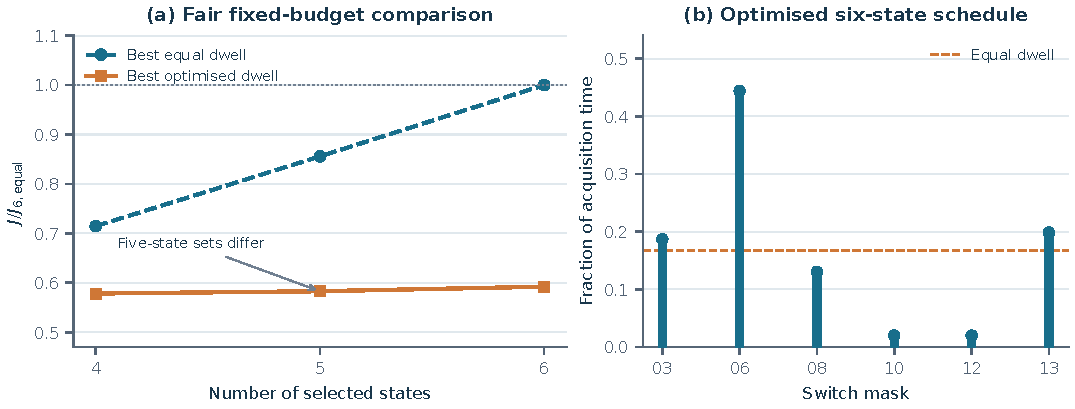
\includegraphics[width=.87\textwidth]{V44_FIXED_BUDGET.pdf}
\caption{Fixed-budget comparison of four-, five- and six-state C033 schedules at 1.925~GHz. (a) Best subset under equal or optimised dwell, normalised to equal-time six-state operation. (b) A-optimal dwell fractions for the full six-state set. Independent equal raw-output noise per unit integration time is assumed.}\label{fig:fixedbudget}
\end{figure*}

For the full set, equal dwell gives $J_T=1764.54$ in arbitrary inverse-gain units and the optimised schedule gives $1044.82$, a 40.8\% reduction. The four-state set $\{03,06,08,13\}$ achieves $J_T=1020.33$ with approximately 19.4\%, 45.7\%, 14.7\% and 20.2\% of the budget assigned to its four masks. Its modest advantage over the constrained six-state schedule comes from avoiding minimum-dwell allocation to less informative states. This result is \emph{not} an accuracy prediction for a vapour-cell experiment: real switching dead time, correlated noise and drift can change the optimum. It does show that information quality and acquisition cost can be optimised together using the existing complex HFSS results, providing a practical state-selection criterion beyond rank and $\kappa_2$.

\subsection{Circular-channel strength and a projected angular-uncertainty bound}
The weakest singular direction of a finite receiving matrix is not necessarily identical to the circular Stokes axis. Nevertheless, the two archived 1.850-GHz, 5-mm finite matrices expose a particularly weak circular coefficient: $\max_k |\widetilde A_{k3}|=0.191$ (P24) and $0.174$ (P27), versus corresponding maximal linear-$S_1$ coefficients $0.972$ and $0.967$. These are direct instrument-matrix diagnostics, rather than a new electromagnetic solve. For any assumed independent equal-variance \emph{normalised} observation error $\sigma_y^2$, the unconstrained linear estimate obeys
\begin{equation}
\operatorname{Cov}(\widehat {\boldsymbol S})=\sigma_y^2
(\widetilde A^{\mathsf T}\widetilde A)^{-1},\qquad
\max_{\|\boldsymbol u\|_2=1}\operatorname{Var}(\boldsymbol u^{\mathsf T}\widehat{\boldsymbol S})=
\frac{\sigma_y^2}{\sigma_{\min}^2(\widetilde A)}.
\label{eq:access_noise_bound}
\end{equation}
For $\sigma_{\min}=0.1412$ (P24) and $0.1247$ (P27), the respective worst-direction standard-deviation amplifications relative to $\sigma_y$ are $7.08$ and $8.02$. These coefficients quantify conditioning \emph{only under the stated hypothetical measurement model}; they are not experimental polarisation errors. If $\boldsymbol s$ and $\widehat{\boldsymbol s}$ are both projected onto the unit Poincar\'e sphere, their geodesic angle satisfies the exact relation
\begin{equation}
\Delta\psi=2\sin^{-1}\!\left(\frac{\|\widehat{\boldsymbol s}-\boldsymbol s\|_2}{2}\right),
\quad \|\widehat{\boldsymbol s}-\boldsymbol s\|_2\le 2.
\label{eq:access_angle}
\end{equation}
This converts a \emph{known} normalised-Stokes perturbation into an angular error without pretending that the HFSS record contains optical readout noise. The finite-channel result suggests a more relevant follow-on objective than reducing $\kappa_2$ alone:
\begin{equation}
\max_{g,\mathcal K}\ \min_{f\in\mathcal B}
\left\{\sigma_{\min}\big[\Sigma_m(f)^{-1/2}A(f;g,\mathcal K)\big]\right\}
\label{eq:access_design}
\end{equation}
subject to fabrication and switching constraints, where $g$ denotes geometry and $\mathcal K$ the selected switch masks. This is a \emph{proposed} receiver-aware optimisation law derived from the present analysis, not an optimisation claimed to have been performed. Adding more masks can improve information if their responses are independent and their noise is modelled consistently; rank alone does not guarantee a useful circular channel.

\subsection{What independent mesh agreement actually supports}
The native HFSS archive also contains two separately adapted periodic meshes across selected L-band frequencies. Figure~\ref{fig:v41_dualmesh} reports their condition-number trajectories without conflating a screening result with a verified operating band. C033 passes the archived dual-mesh criteria at 1.925 and 1.950 GHz, among other sampled points, whereas intervening frequencies can fail additional acceptance gates even when both condition numbers appear favourable. The screening interval of 250 MHz is therefore an optimisation metric on its discovery grid, not a proven continuous 250-MHz fabrication specification. This qualification matters when selecting the exact carrier and switching schedule for a fixed-frequency prototype.

\begin{figure*}[t]
\centering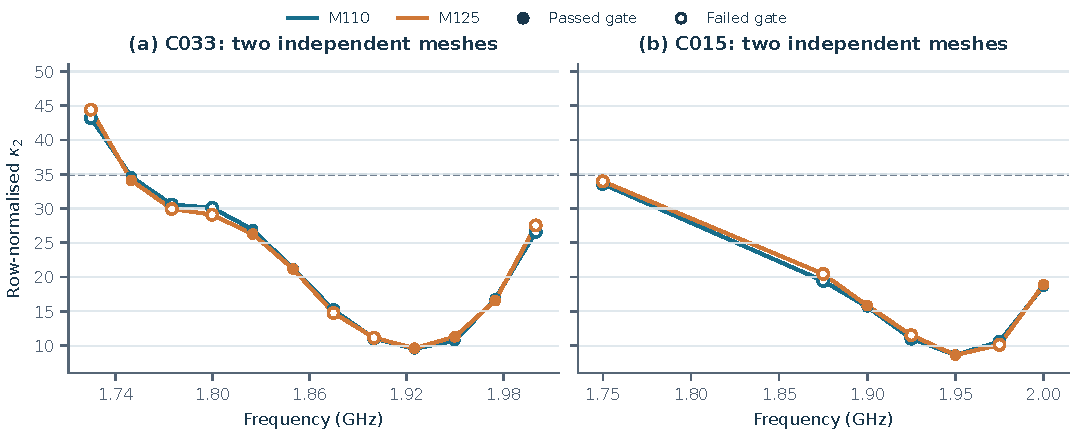
\includegraphics[width=.89\textwidth]{V41_FIG_INDEPENDENT_HFSS_PASS.pdf}
\caption{Independently adapted periodic HFSS results for C033 and C015. Filled markers identify frequencies satisfying the archived full dual-mesh verification gate; open markers indicate a failed gate. The dotted line shows the nominal conditioning threshold.}\label{fig:v41_dualmesh}
\end{figure*}


\section{Finite-Aperture Check and Manufacturing Outlook}
\subsection{Finite-aperture behaviour}
A distinct 82$\times$82-mm $3\times3$ model was examined at 1.850 GHz, using two orthogonal incident fields and six conductor masks. The sampled receiving region was 70$\times$50 mm at planes 5--50 mm behind the board. Both completed mesh policies yielded rank-four receiving matrices. At the nearest 5-mm plane, their row-normalised condition numbers were 24.72 and 21.93: the finite geometry still responds differently to all four Stokes coordinates, but its weakest direction is less robust than the periodic model at 1.925~GHz. The 6.18\% intermesh matrix difference shows that the calculated local receiving fields are also more sensitive to numerical refinement. Rank four and condition numbers below the project screening threshold are therefore promising evidence of \emph{observability}, but do not prove accurate finite-board \emph{calibration transfer}. The complete conditioning-versus-distance and deterministic transfer analysis is presented in Appendix~\ref{app:finite}. The distinction between \emph{observable} and \emph{calibration-stable} is important when extrapolating from a periodic surface to a small receiver.

\subsection{Printed-board implementation}
The native HFSS layout fixes a 24-mm periodic cell with two patterned copper faces on one 1.6-mm dielectric layer. In the selected C033 geometry the front and rear nominal trace widths are 1.400 and 1.106 mm, respectively, and the nominal switch gap is 1.887 mm (parameter-table values). These dimensions are compatible in principle with conventional two-sided PCB patterning and provide a concrete starting point for fabrication drawings. However, manufacturability additionally requires final CAD/DRC validation of every copper clearance and minimum feature, via/drill and solder-pad definition, and suitable dielectric and copper stack-up tolerances.

\begin{table}[t]
\caption{Nominal HFSS layout of selected candidate C033}
\label{tab:pcb_specs}
\centering\footnotesize
\begin{tabular}{@{}ll@{}}
\toprule
Parameter & Design value \\
\midrule
Periodic pitch & 24 mm \\
Dielectric thickness & 1.60 mm \\
Front conductor width & 1.400 mm \\
Rear conductor width & 1.106 mm \\
Nominal switch gap & 1.887 mm \\
Finite array & $3\times3$ cells; 82-mm board \\
State selectors & Four ideal conducting bridges \\
\bottomrule
\end{tabular}
\end{table}

The HFSS campaign toggled ideal conductor bridges. Real PIN diodes add series resistance, package inductance, off-state capacitance, bias feeds and solder-pad discontinuities; therefore the exact measured condition number and transmission of a fabricated board cannot be inferred without updating and revalidating the network. The physically justified engineering expectation is that the patterned conductor topology can be fabricated and its switch states can generate distinct RF responses, while their achieved bandwidth, insertion loss and inverse conditioning remain measurable design targets. The surface's verified contribution is the simulated, independently checked periodic analyser rather than a fabricated performance specification.

\section{Discussion: What the electromagnetic results establish}
A full-rank instrument is necessary for full-Stokes analysis, but it does not establish reliable reconstruction. Consider two matrices with rank four: if one has a very small fourth singular value, a small change in field response can generate a much larger change in its inferred Stokes vector. The selected periodic design achieves $\kappa_2(\widetilde A)=9.53$ at 1.925 GHz, markedly better conditioned than the $34.62$ value reported at 1.750 GHz for the same geometry. In a worst-case relative perturbation \emph{bound}, 9.53 multiplies the small-error term instead of 34.62. These are sensitivity bounds, not expected percentage errors and not experimental accuracies. The 0.551\% independently adapted matrix disagreement at 1.925 GHz provides separate evidence that this particular periodic calculation is numerically consistent.

Switch-state diversity and received power must then be considered together. Mask 06 is essential to the least-observed Stokes direction in the archived periodic instrument yet has relatively low raw gain. The gain-aware and fixed-budget analyses demonstrate that a reduced condition number alone need not minimise total inverse-estimator uncertainty. Under the declared independent, time-scaled variance model, allocating dwell according to information reduces the six-state inverse-trace criterion by 40.8\%. This result is a conditional algorithmic design rule, not a measured improvement in atomic signal-to-noise ratio. It also motivates a practical prototype test: preserve the configurations that supply independent circular information and characterise their actual RF loss before choosing a switching schedule.

The finite-panel calculation draws the clearest boundary around the claim. An $82\times82$-mm array retains rank four near the receiving plane, but its weak circular coefficient and mesh-dependent calibration transfer prevent transfer of the favourable periodic condition number into a demonstrated hardware accuracy specification. A matched-frequency, matched-aperture comparison against a published programmable RF polarimeter \cite{Chen2025Reconfigurable} is likewise still needed before claiming comparative superiority. Taken together, the data demonstrate an independently checked \emph{periodic electromagnetic analyser}, quantify the value of its switching states and identify the specific numerical risks that govern integration into a finite Rydberg-compatible instrument.

\section{Conclusion}
\noindent\textbf{Achievements.} We designed a two-face, switch-programmable microwave metasurface and developed a six-state Jones-to-Stokes measurement method using its complex HFSS response. Among 36 candidate geometries, the longest accepted sampled interval increased from 175 to 250 MHz. At 1.925 GHz the selected periodic model is rank four, $\kappa_2(\widetilde A)=9.53$, and the independently adapted instruments differ by 0.551\%. A state-information analysis further demonstrates how polarisation diversity, raw receiving gain and a fixed integration-time budget affect the choice of useful switching configurations.

\noindent\textbf{Limitations.} The continuous bandwidth and fabricated switch response have not been validated. The finite $3\times3$ instrument retains algebraic observability but gives weaker circular sensitivity and substantially poorer cross-mesh calibration transfer. The original measured linear-polariser contrast belongs to a different experimental fixture and does not independently validate full-Stokes performance of the simulated PCB.

\noindent\textbf{Future work.} The next design iteration should independently converge the finite receiving operator at the same frequency as the periodic optimum, strengthen the circular channel, and include characterised PIN-diode and bias-line parasitics before PCB fabrication. Calibrated RF and later transition-specific optical measurements can then test the information-derived switching schedules. The result established here is a reproducible electromagnetic design method and a verified periodic measurement basis, with a concrete experimental programme to evaluate its real-world accuracy.



\appendix
\section{Finite Array and Calibration-Transfer Diagnostics}\label{app:finite}
\subsection{Poincar\'e-sphere reconstruction and calibration transfer}
The six-state Jones transmission coefficients define an $A\in\mathbb R^{6\times4}$ instrument for each RF model and frequency. Evaluating 1,231 test states against one matrix and inverting the outputs using that same matrix verifies the algebra and basis conventions, but cannot quantify independent calibration accuracy. We therefore use a distinct test: a reconstructed Stokes vector is inferred with one independently meshed finite HFSS instrument while its nominal response is generated using the second finite HFSS instrument.

At the 5-mm receiver plane and 1.850 GHz, the completed P24 and P27 copper-mesh policies both yield rank four; their respective \emph{row-gain-normalised} condition numbers are 21.93 and 24.72 (raw-matrix conditions 21.15 and 26.91). Using 1,231 deterministic fully polarised states uniformly sampled on the Poincar\'e sphere, $\mvec_{\mathrm{P27}}=A_{\mathrm{P27}}\Svec$ was inverted using $A_{\mathrm{P24}}^{+}$, and vice versa. With the explicitly defined full-vector error $100\|\widehat\Svec-\Svec\|_2/\|\Svec\|_2$, the P24-calibrated/P27-observed direction gives a 95th percentile of 156.8\% and maximum of 165.2\%; the reverse direction gives 72.2\% and 76.6\%. These values follow directly from the archived $6\times4$ matrices and are a new offline numerical post-processing test, not new HFSS solves. Errors greater than 100\% are possible because the estimator is an unconstrained linear pseudoinverse and the error metric is a norm of the full four-vector rather than a bounded polarisation-angle error.

\begin{figure*}[t]
\centering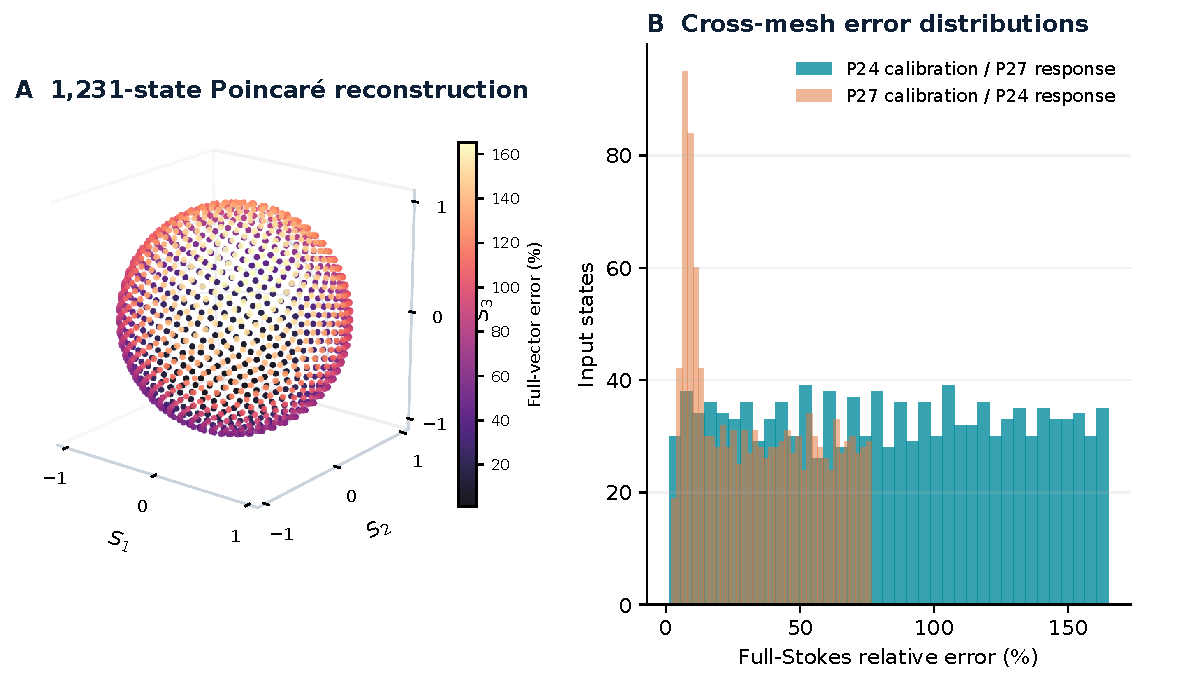
\includegraphics[width=.92\textwidth]{FINAL_F09_STOKES_AB_VECTOR.pdf}
\caption{Finite-array cross-mesh Stokes reconstruction and calibration-transfer errors at 1.850 GHz, 5 mm.}\label{fig:polsphere}
\end{figure*}

The result is revealing: polarisation sensitivity and rank-four observability are already present, while quantitative finite-aperture calibration transfer remains sensitive to the calculated receiving fields. The published-periodic best point at 1.925 GHz and the finite test at 1.850 GHz also answer different simulation questions, so their respective condition numbers are displayed as separate validation stages rather than an assumed finite-board reproduction of the periodic optimum.
\subsection{Finite electromagnetic experiment}
The optimised split-loop was assembled into a $3\times3$, 82-by-82-mm finite electromagnetic model at 1.850~GHz, with plane-wave excitation under the two orthogonal input axes. Six ideal switch states give twelve HFSS patterned cases. The finite receiver was evaluated by integrating the squared transverse field over the sampled 70-by-50-mm receiving region, on planes 5, 10, 20 and 50~mm behind the panel. Incident, scattered and total field exports were separately identified, with total fields used for the final receiver calculations.

\subsection{Six-state observability and distance dependence}
The resulting receiving matrices are rank four under both completed HFSS mesh policies. On the 2.7-mm local copper mesh the normalised condition numbers at the four receiver planes are 24.72, 24.82, 59.81 and 209.15; on the 2.4-mm mesh they are 21.93, 30.17, 61.37 and 176.74. Figure~\ref{fig:finitecond} presents the distance dependence most relevant to placement and numerical stability. The strongest polarimetric separability occurs close to the surface, within the simulated 5--10-mm observation interval.

\begin{figure}[tb]
\centering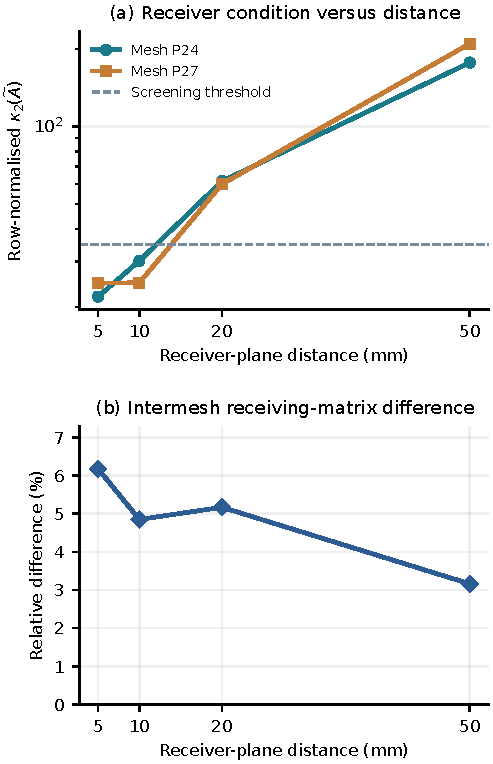
\includegraphics[width=.97\columnwidth]{FINAL_F10_FINITE_DISTANCE.pdf}
\caption{Finite HFSS receiver-distance dependence at 1.850 GHz, presented within a single column as vertically stacked subplots: (a) row-normalised condition number and (b) intermesh receiving-matrix difference. Both meshes retain rank-four receiving operators at all displayed planes.}\label{fig:finitecond}
\end{figure}

The trend is physically useful: finite-aperture near-fields and spatially varying polarisation generally relax toward a more uniform transmitted field as the observer moves away from the patterned surface. That propagation changes the diversity among switched RF states. As a result, a metasurface optimised using an infinite periodic far-field Jones matrix is not automatically optimal for a finite, spatially averaged atomic receiving volume.

\subsection{Which Stokes coordinates constrain the finite design?}
The full-rank test answers whether all four Stokes coordinates are algebraically identifiable, but it does not quantify how evenly the basis spans the Poincar\'e sphere. Define the row-normalised instrument \(\widetilde A\) by \(\widetilde A_{kj}=A_{kj}/A_{k0}\). Singular-value decomposition of the two archived finite receiving matrices at 1.850 GHz and 5 mm gives the independent diagnostic in Fig.~\ref{fig:svd}. The smallest singular values are 0.1412 (P24) and 0.1247 (P27), compared with largest values of 3.0976 and 3.0821. The maximum absolute normalised \(S_3\)-coefficient is respectively 0.191 and 0.174, whereas the maximum \(S_1\)-coefficient is 0.972 and 0.967. Thus the finite implementation is observably more responsive to at least one linear-polarisation axis than to circular quadrature. This is not an extra electromagnetic simulation: the displayed singular spectra are calculated from the two archived six-by-four HFSS receiving matrices. Improving near-cell circular response while preserving full rank is therefore a concrete receiver-aware optimisation requirement.
\begin{figure}[tb]
\centering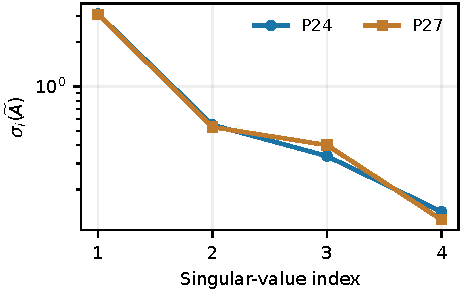
\includegraphics[width=.92\columnwidth]{F11_FINITE_SINGULAR_SPECTRA.pdf}
\caption{Singular values of the \(6\times4\) row-gain-normalised finite Stokes matrices at 1.850 GHz, 5 mm, computed directly from the archived P24 and P27 HFSS receiving data. Smaller fourth singular values identify weaker polarisation directions even though both matrices retain rank four.}\label{fig:svd}
\end{figure}

\subsection{Finite-field mesh comparison}
The two completed finite meshes produce a 6.18\% relative instrument-matrix discrepancy at 5~mm. Calibration of one mesh against the fields computed on the other gives 95th-percentile Stokes-vector discrepancies of 156.8\% (P24 calibration, P27 observations) and 72.2\% in the reverse direction over 1,231 prescribed fully polarised states. The resulting distinction is central: both numerical operators have rank four, while their quantitative cross-mesh transfer differs substantially. Additional targeted HFSS refinement resolved two strict-energy diagnostic cases, but did not produce a complete third converged six-state instrument. Thus finite-array observability is established within the completed calculations; mesh-independent reconstruction accuracy is a separate unresolved numerical criterion.




\subsection{Finite receiving-volume physics and the observation-plane trade-off}
Periodic HFSS Floquet coefficients describe transmission through an infinite array. A real printed panel terminates at its edges, and the resulting field can vary in direction, magnitude and phase across a nearby vapour-cell volume. The finite model thus addresses a different question from the periodic unit-cell response. A finite surface may retain polarisation-selective local fields even when its far-field transmitted beam is less strongly polarisation discriminating; conversely, a periodic model with strong cross-polar transmission does not by itself guarantee useful coupling to a particular finite detector area. The receiving-volume functional makes that distinction explicit.

The finite calculations used separate $x$- and $y$-polarised plane-wave bases. For each state, the complex transverse field at every sample point is a linear combination of these two solutions. Integrating its quadratic receiving-axis magnitude produces the instrument row appropriate to the declared observation plane. This construction is advantageous because a complete state sweep requires twelve physical HFSS cases rather than a separate electromagnetic solve for every incident point on the Poincar\'e sphere. The input-state enumeration used for reconstruction is consequently a transparent mathematical post-processing step.

The 5- and 10-mm planes yield normalized instrument conditions below the predefined threshold on both completed mesh policies. The 20- and 50-mm planes show progressively poorer conditioning, even though the system remains rank four. This distinction is physically informative: algebraic observability and practical robustness are not identical. Near the surface, spatially structured fields can provide stronger differences between switching states; at larger distances, the state responses become closer and the condition number grows. Receiver placement must therefore be included among the RF design variables when the surface is intended to operate beside a small atomic sampling volume.

The remaining numerical qualification concerns the complex fields themselves. Finite-region field quantities can be sensitive to mesh refinement at sharp conductor edges and in strongly varying near-field zones. HFSS adaptive convergence in a global energy quantity cannot automatically certify every receiver-point field. Accordingly, a stronger local field-convergence check must include the complex response at the specified receiving volume, not only a global adaptive energy measure. The present finite simulation establishes the response of the declared numerical models, their distance trends and the sensitivity of calibration transfer to mesh policy.


\section{Atomic Readout as a Separate Transfer Function}\label{app:atom}
\subsection{Four-level transfer law}
The metasurface changes the complex microwave field over the atomic receiving volume. To make the receiver coupling explicit, consider the four-level rubidium EIT ladder $|1\rangle\leftrightarrow|2\rangle\leftrightarrow|3\rangle\leftrightarrow|4\rangle$, where the final coupling is microwave-driven. At switch state $k$ and location $\mathbf r$, the RF Rabi coupling is
\begin{equation}
\Omega_{\rm RF,k}(\mathbf r)=\frac{|\mathbf d_{34}\cdot\mathbf E_k(\mathbf r)|}{\hbar}.
\label{eq:opticalbridge}
\end{equation}
In the weak-probe steady-state approximation, the velocity-resolved susceptibility can be represented using complex detuning/decay coefficients $d_{21}(v),d_{31}(v),d_{41}(v)$ as
\begin{equation}
\chi_{k,v}(\Delta_p,\mathbf r)=
\frac{\mathrm i\chi_0}{d_{21}(v)+\dfrac{|\Omega_c|^2}{4\left[d_{31}(v)+\dfrac{|\Omega_{\rm RF,k}(\mathbf r)|^2}{4d_{41}(v)}\right]}}.
\label{eq:fourlevel}
\end{equation}
Here $\chi_0$ is proportional to the optical transition strength and atomic density, while the complex $d_{ij}$ include optical and microwave detunings, decoherence, and Doppler shifts according to the selected ladder and velocity convention. This compact four-level transfer form is consistent with the independently supplied rubidium-receiver theory\cite{Somaweera2025Review}; it is a useful physical model rather than an optical fit to the HFSS data.

Let $F_T(v)$ be the normalised thermal velocity distribution. For a specified optical transverse mode with normalized power weight $W_\perp(\boldsymbol\rho)$, a propagation-sensitive transmission model is
\begin{equation}
\begin{split}
T_k(\Delta_p)&=\int d^2\boldsymbol\rho\,W_\perp(\boldsymbol\rho)\\
&\times\exp\!\Bigg[-k_p\int_0^L dz\;\operatorname{Im}
\left\{\int dv\,F_T(v)\chi_{k,v}\right\}\Bigg],
\end{split}
\label{eq:opticalvolume}
\end{equation}
Equation~\eqref{eq:opticalvolume} explicitly separates spatial optical averaging, Doppler averaging, and nonlinear field-to-transmission coupling. Its geometry and local $\mathbf E_k(\mathbf r)$ are supplied by the finite HFSS model; its atomic constants, transition selection and fit protocol must be fixed before deriving a predicted measured Stokes error. The matrix $A$ used throughout this paper corresponds to the independently defined RF quadratic proxy, $m_k=\int w|\mathbf e_d\cdot\mathbf E_k|^2dV$. Only when the extracted optical feature is calibrated to be proportional to that proxy can $\mvec=A\Svec$ be applied directly to the atomically measured channel.

For a resolved, on-resonance Autler--Townes doublet of approximately uniform microwave coupling, the usual local relation is
\begin{equation}
\Delta f_{{\rm AT},k}\approx |\mathbf d_{34}\cdot\mathbf E_k|/h.
\label{eq:atsplittransfer}
\end{equation}
For a spatially nonuniform illuminated ensemble, the splitting extracted from an averaged spectrum need not equal the square root of the volume-average squared field. The coupled equations above show which approximation must be tested to turn the present electromagnetic analyser into a full optical polarimeter, without reinterpreting a local HFSS receiving power as a measured atomic observable.

\subsection{Local optical sensitivity and information transfer}
The nonlinear atomic transfer model provides a controlled path to an optical version of the electromagnetic receiving matrix. Put $q_k(\mathbf r)=|\mathbf d_{34}\cdot\mathbf E_k(\mathbf r)|^2/\hbar^2$, and let $\mathcal T_k(\Delta_p;\{q_k\})$ denote the Doppler- and mode-integrated transmission in Eq.~\eqref{eq:opticalvolume}. For a selected operating spectrum, a first-order variation about an established RF operating field $q_k^{(0)}$ gives
\begin{equation}
\delta T_k(\Delta_p) =\int_{\Vroi} K_k(\mathbf r;\Delta_p)\,\delta q_k(\mathbf r)\,dV+O(\|\delta q_k\|^2),
\label{eq:optical_kernel}
\end{equation}
where $K_k=\delta\mathcal T_k/\delta q_k$ is the functional sensitivity of the \emph{optical} readout. Its sign and spatial variation depend on optical detuning and the atomic operating point. When this sensitivity is approximately constant over the interrogated region, or can be independently calibrated into an appropriate spatial weight, the optical differential measurements inherit the same bilinear Jones structure and admit a local $6\times4$ effective Stokes Jacobian. Otherwise the complete optical model must be inverted rather than applying the HFSS-only matrix directly. This distinction gives a quantitative criterion for transferring the electromagnetic analyser to the actual receiver.

For calibrated measurement covariance $\Sigma_m$, the corresponding local Fisher-information matrix is
\begin{equation}
\mathcal I_S=A_{\rm opt}^{\mathsf T}\Sigma_m^{-1} A_{\rm opt},\quad
 \mathrm{Cov}(\widehat{\boldsymbol S})\succeq\mathcal I_S^{-1},
\label{eq:fisher}
\end{equation}
under a regular unbiased Gaussian-response approximation. Thus the smallest eigenvalue of $\mathcal I_S$ expresses the least-observed Stokes direction and the determinant measures four-dimensional information volume. The inverse bound is statistical and is \emph{not} assigned a numerical detector-noise value in the HFSS study. It nevertheless establishes a precise route from the full-wave complex fields, via atomic susceptibility, to a sensitivity-calibrated figure of merit for subsequent optical operation.


\section{Receiving-Operator Derivations and Verification}\label{sec:derived}

\subsection{Incident field convention and calibrated observables}
Let a quasi-monochromatic incident field of fixed propagation direction have transverse Jones vector $\boldsymbol{j}=(a,b)^{\mathsf{T}}$. We use the Stokes convention
\begin{subequations}\label{eq:stokes}
\begin{align}
S_0&=|a|^2+|b|^2, & S_1&=|a|^2-|b|^2,\\
S_2&=2\Re(a^*b), & S_3&=-2\Im(a^*b).
\end{align}
\end{subequations}
The sign of $S_3$ is a declared convention chosen to match the complex phasing of the HFSS post-processing code. Consequently, circular-handedness labels must be read together with the propagation and time-harmonic conventions. For fully polarized states $S_1^2+S_2^2+S_3^2=S_0^2$; partially polarized states lie inside the normalized Poincar\'e sphere. Equation~(\ref{eq:stokes}) is established polarimetry, not an original theorem of this project.

At a given frequency $f$ and switch state $k$, denote the HFSS complex electric-field component along the selected receiving axis by $u_k(\boldsymbol{r};f)$ for an incident unit-amplitude $x$ basis and $v_k(\boldsymbol{r};f)$ for the orthogonal $y$ basis. For a linear, time-invariant structure with the same material state and mesh, superposition gives
\begin{equation}
E_{x,k}(\boldsymbol{r};f)=a\,u_k(\boldsymbol{r};f)+b\,v_k(\boldsymbol{r};f).
\label{eq:superposition}
\end{equation}
The idealized scalar observation is a nonnegative, spatially weighted field magnitude,
\begin{equation}
m_k(f)=\int_{\Vroi}w(\boldsymbol{r})\,\big|E_{x,k}(\boldsymbol{r};f)\big|^2\,\mathrm{d}V,
\quad \int_{\Vroi}w\,\mathrm{d}V=1,
\label{eq:observable}
\end{equation}
where $w\ge0$ represents a specified receiving-volume sampling rule. In the principal numerical model, the available discrete field grid was uniformly weighted; a narrower central Gaussian weighting was considered separately. This is a modeled electromagnetic \emph{intensity proxy}, not a calibrated Rydberg optical-signal law. It provides a physically admissible field projection for optimising analyser diversity; optical observables require the atomic susceptibility and its spatial averaging to be independently specified.

Define three complex-field integrals
\begin{align}
P_k&=\int w|u_k|^2\,\mathrm{d}V,\quad Q_k=\int w|v_k|^2\,\mathrm{d}V,\notag\\
C_k&=\int w u_k^*v_k\,\mathrm{d}V.
\label{eq:overlaps}
\end{align}
Inserting Eq.~(\ref{eq:superposition}) into Eq.~(\ref{eq:observable}), and using $a^*b=(S_2-\cpx S_3)/2$, yields
\begin{equation}
\boxed{\begin{aligned}
m_k={}&\tfrac12(P_k+Q_k)S_0+\tfrac12(P_k-Q_k)S_1\\
&+\Re(C_k)S_2+\Im(C_k)S_3.
\end{aligned}}
\label{eq:operator}
\end{equation}
The six-state instrument is therefore $\mvec=\Avec\Svec+\boldsymbol{\epsilon}$, where row $k$ of $\Avec$ is precisely the four coefficients in Eq.~(\ref{eq:operator}). We stress the scope of this derivation. It is an exact identity for the declared linear electromagnetic response and spatially integrated quadratic observable, not an assertion that the switched surface creates an ideal waveplate or that $\epsilon$ has a known laboratory distribution.

\subsection{Positive-semidefinite receiving operators and physical admissibility}
At each switch state the two complex basis fields define a $2\times2$ Hermitian Gram matrix
\begin{equation}
\mathbf{G}_k=\begin{pmatrix}P_k&C_k\\C_k^*&Q_k\end{pmatrix}\succeq0.
\label{eq:gram}
\end{equation}
Cauchy--Schwarz implies $|C_k|^2\le P_kQ_k$. In Stokes coordinates, this enforces
\begin{equation}
A_{k0}\ge\sqrt{A_{k1}^2+A_{k2}^2+A_{k3}^2},
\label{eq:bound}
\end{equation}
provided the indices $0,1,2,3$ refer to the columns defined above. Thus every physical row lies in the Lorentz-like positive cone of nonnegative polarization analyzer responses; a numerical candidate violating Eq.~(\ref{eq:bound}) indicates an extraction or convention fault, not exceptionally good polarization sensitivity. The inequality is a standard consequence of positive semidefinite coherency/Gram matrices\cite{Azzam1990}; the application-specific aspect here is its evaluation directly from the local HFSS field integrals.

For channel-to-channel comparison, define $\widetilde A_{kj}=A_{kj}/A_{k0}$ whenever $A_{k0}>0$. This operation factors out each state's total gain and reveals its normalized polarization analyzer vector $\boldsymbol{p}_k=(\widetilde A_{k1},\widetilde A_{k2},\widetilde A_{k3})$. The bound above becomes $\norm{\boldsymbol{p}_k}_2\le1$. In particular, $\eta_3=\max_k|\widetilde A_{k3}|$ is a convenient circular-Stokes \emph{sensitivity coefficient}, but it is not circular dichroism, handedness extinction, or Stokes reconstruction precision. Maximizing $\eta_3$ alone can worsen the independence of the four analyzer vectors.

\subsection{Affine-span test for analyser observability}
For each state with \(A_{k0}>0\), introduce a three-component normalised analyser vector \(\boldsymbol p_k=(A_{k1},A_{k2},A_{k3})/A_{k0}\). The corresponding instrument row is \(A_{k0}(1,\boldsymbol p_k^{\mathsf T})\). Multiplying by the invertible diagonal gain matrix \(\operatorname{diag}(A_{10},\ldots,A_{60})\) does not alter rank, hence
\begin{equation}
\boxed{\operatorname{rank}(A)=4\iff\dim\operatorname{aff}\{\boldsymbol p_1,\ldots,\boldsymbol p_6\}=3.}
\label{eq:affine}
\end{equation}
To prove the reverse implication, subtract the first normalised row from the other rows. The remaining lower block is precisely the matrix of differences \(\boldsymbol p_k-\boldsymbol p_1\); it has rank three exactly when the six polarimetric analyser points do not lie in an affine plane. The first homogeneous coordinate supplies the fourth dimension. This reformulation makes the difference between full-Stokes observability and simple cross-polar attenuation geometrically explicit; it does not assume an ideal tetrahedral instrument.

\subsection{Observability, conditioning and uncertainty transfer}
The six-state instrument $\Avec\in\mathbb R^{6\times4}$ has four independently identifiable Stokes coordinates when $\operatorname{rank}(\Avec)=4$. For an arbitrary positive-definite measurement weighting $W$, define the rectangular least-squares reconstruction operator
\begin{equation}
L_W(\Avec)=(\Avec^{\mathsf T}W\Avec)^{-1}\Avec^{\mathsf T}W,\quad
\widehat{\Svec}=L_W(\widehat{\Avec})\mvec.
\label{eq:weightedls}
\end{equation}
For the deterministic tests reported here $W=I$ and the inverse was calculated using a singular-value decomposition. With actual measured covariance $\Sigma_m$ one can instead use $W=\Sigma_m^{-1}$ when the corresponding statistical model is justified. Defining $\widehat{\Avec}=\Avec+\Delta\Avec$ and $\mvec=\Avec\Svec+\boldsymbol\epsilon$, the full-column-rank identity $L_W(\widehat\Avec)\widehat\Avec=I$ yields
\begin{equation}
\boxed{\widehat{\Svec}-\Svec=
L_W(\widehat{\Avec})(\boldsymbol\epsilon-\Delta\Avec\Svec).}
\label{eq:perturb}
\end{equation}
Consequently,
\begin{equation}
\|\delta\Svec\|_2\le\|L_W(\widehat\Avec)\|_2\left(
\|\boldsymbol\epsilon\|_2+\|\Delta\Avec\|_2\|\Svec\|_2\right).
\label{eq:errorbound}
\end{equation}
When the calibrated matrix is fixed, the first-order measurement covariance is
\begin{equation}
\Sigma_S\simeq L_W(\Avec)\,\Sigma_m\,L_W(\Avec)^{\mathsf T},
\label{eq:covariance}
\end{equation}
with separate terms needed for matrix uncertainty. No detector-noise statistics are inferred from the purely electromagnetic archive. Row-normalised matrices are useful for shape/condition screening, but their use for inversion requires scaling the observation vector by the identical row gains. All new finite cross-mesh tests instead use the complete stored, unnormalised instrument matrices.

The geometric viewpoint is equally useful. Four normalized analyzer vectors define a tetrahedron inside the Poincar\'e unit ball. If their points approach a plane, the smallest singular value collapses and at least one Stokes direction becomes poorly observable; tetrahedral design and conditioning are established polarimetry concepts\cite{Tyo2002,Azzam1988}. We use these principles as design diagnostics. Near-field mesh transfer is quantitatively distinct from a within-mesh condition number.

\subsection{Independent-source verification of the Stokes algebra}
The native Floquet responses provide a direct numerical test of the field-overlap equations rather than simply a conceptual Poincar\'e construction. At 1.825 GHz, an archived C000 screening case was independently reprocessed from its simulated complex Jones coefficients to evaluate the Gram-to-instrument identity, circular interference coefficient, and numerical pseudoinverse over 1,231 prescribed incident states. Table~\ref{tab:equation-validation} reports the largest residuals. These near-roundoff values establish consistency of the mathematical transformations applied to HFSS outputs; they are not independent electromagnetic reruns or measurements of hardware accuracy.
\begin{table}[tb]
\caption{HFSS-source equation checks (C000, 1.825 GHz).}
\label{tab:equation-validation}
\centering\small
\begin{tabular}{@{}lr@{}}
\toprule
Test & Maximum residual\\
\midrule
Receiving-operator identity & $4.44\times10^{-16}$\\
Circular-response identity & $2.22\times10^{-16}$\\
1,231-state algebraic reconstruction & $9.67\times10^{-15}$\\
\bottomrule
\end{tabular}
\end{table}
This result complements the independently adapted C033 periodic mesh comparison: the former tests analytical implementation, whereas the latter tests numerical stability of electromagnetic fields. Both are needed to support an accurate simulation-first conclusion.


\subsection{Derived design tests: admissibility, information bandwidth, and calibration transfer}
The field-overlap construction supplies three directly checkable results for candidate screening. First, Cauchy--Schwarz forces each gain-normalized analyser row to remain inside the unit Poincar\'e ball [Eq.~(\ref{eq:bound})]; this is an extraction-consistency test, not a new universal physical law. Second, the frequency-domain \emph{nominal information set} for thresholds $\kappa_{\max}$ and $\eta_{\min}$ is
\begin{equation}
\begin{split}
\mathcal B_{\rm nom}=\{f:\;&\operatorname{rank} A(f)=4,\\
&\kappa_2(\widetilde A(f))\le\kappa_{\max},\ \eta_3(f)\ge\eta_{\min}\}.
\end{split}
\label{eq:bandgate}
\end{equation}
A connected component of $\mathcal B_{\rm nom}$ is only a \emph{candidate} information bandwidth; measured sensitivity, finite-board transmission and independent-mesh agreement are additional necessary tests. Third, Eq.~(\ref{eq:errorbound}) provides an exact algebraic route from calibration drift to an error bound. These relationships were checked against archived finite complex-field data and synthetic Jones vectors. Their novelty is their particular combination in a receiver-aware HFSS screening workflow, not the underlying algebra of Stokes vectors, matrix norms or positive semidefinite quadratic forms.


\subsection{Derived equator restriction error and ideal analyser conditioning}
Two analytical baselines are useful in interpreting the early partial-Stokes estimates. Let a fully polarized state have azimuth $\psi$ and ellipticity angle $\chi\in[-\pi/4,\pi/4]$. Its normalized Stokes vector can be written $\boldsymbol s=(\cos2\chi\cos2\psi,\cos2\chi\sin2\psi,\sin2\chi)$. A procedure that forces $S_3=0$ and projects the measured vector onto the nearest equatorial direction incurs the geodesic angular separation
\begin{equation}
\epsilon_{\rm lin}=\cos^{-1}(\cos 2\chi)=2|\chi|,\quad |\chi|\le\pi/4,
\label{eq:linear_error}
\end{equation}
where the angle is a \emph{Poincar\'e-sphere angular error}, not a physical antenna pointing angle. The relation follows directly from the inner product of the normalized state and its equatorial projection, and assumes full polarization. It quantifies the consequence of ignoring an unmeasured circular coordinate even when the linear components have been determined exactly. The 0.887 linear-Stokes magnitude reported in the historical estimate does not establish whether the remainder is circularly polarized or partially polarized: therefore Eq.~(\ref{eq:linear_error}) must not be used to assign a unique historical $\chi$.

A second analytic benchmark is the tetrahedral four-analysis instrument. Take four unit analyzer vectors $\boldsymbol n_k$ that satisfy $\boldsymbol n_i\cdot\boldsymbol n_j=-1/3$ for $i\ne j$ and define ideal equally weighted rows $a_k=\tfrac12(1,\boldsymbol n_k^{\mathsf T})$. Then $A^{\mathsf T}A=\mathrm{diag}(1,1/3,1/3,1/3)$ and
\begin{equation}
\kappa_2(A_{\rm tetra})=\sqrt{3}.
\label{eq:tetra}
\end{equation}
The equality is established polarimeter theory and here serves solely as a transparent mathematical comparator. Suppressing the circular coordinates of the analyzer vectors collapses the smallest singular value and eventually the matrix rank. Thus a nominal rank-four matrix with a very small singular value is not close to a tetrahedral instrument just because all four Stokes coefficients are nonzero. The numerical benchmarks are reproducible from these expressions and the archived analysis script.



\subsection{Finite-aperture electromagnetic scaling}
The finite panel couples a bounded transverse footprint to a local receiver. Two independent dimensionless ratios specify distinct finite-size regimes: the electrical aperture $D/\lambda_0$ and the observation-plane Fresnel number $N_F=D^2/(\lambda_0 z)$, with $\lambda_0=c/f$. At $f=1.85\,{\rm GHz}$, $\lambda_0\simeq162\,{\rm mm}$; the modelled $D=82\,{\rm mm}$ therefore has $D/\lambda_0\simeq0.51$. An ideal infinite-sheet Floquet transmission coefficient need not directly predict the total field sampled over a finite $70\times50\,{\rm mm}^2$ region.

For the four observation planes used in the finite HFSS analysis, the corresponding geometric Fresnel numbers \(N_F\) at 1.85 GHz are approximately 8.30, 4.15, 2.07 and 0.83 for \(z=5,10,20,50\) mm. These numbers characterize source-to-receiver geometry; they are not fitted diffraction efficiencies or estimates of polarimetric accuracy. 

This distinction can be seen without assuming any empirical diffraction fit. In an aperture-equivalence description, the received field is an integral over equivalent electric and magnetic currents $\mathbf J_s,\mathbf M_s$ on the finite surface,
\begin{equation}
\mathbf E(\mathbf r)=\int_{\mathcal A}\left[\overline{\mathbf G}_{EJ}(\mathbf r,\mathbf r')\mathbf J_s(\mathbf r')+\overline{\mathbf G}_{EM}(\mathbf r,\mathbf r')\mathbf M_s(\mathbf r')\right]dA',
\label{eq:finite_aperture}
\end{equation}
where the dyadic Green functions account for free-space propagation and edge diffraction. For any finite $D$, both the observation distance and the illuminated region influence the integrated receiving operator. This explains why the periodic and $3\times3$ finite HFSS matrices are not simply interchangeable, and why the receiving-plane dependence reported here is a genuine part of the engineered polarimeter rather than a plotting choice.

\section*{Nomenclature}
\small\noindent\begin{tabularx}{\columnwidth}{@{}lX@{}}
$\boldsymbol j=(a,b)^\mathrm T$ & Incident Jones vector in the declared $x,y$ basis\\
$\boldsymbol S=(S_0,S_1,S_2,S_3)^\mathrm T$ & Incident Stokes vector; $S_3$ uses the stated harmonic convention\\
$J_k,\boldsymbol t_k$ & Complex Jones transmission matrix and selected output row, mask $k$\\
$A,\widetilde A$ & Six-state instrument and its row-gain-normalised form\\
$\mathbf H_k,\mathbf G_k$ & Positive-semidefinite receiving and Gram operators\\
$m_k,\boldsymbol m$ & Modelled quadratic field response and six-element measurement vector\\
$\boldsymbol p_k$ & Normalised three-component Poincar\'e analyser vector\\
$\sigma_i,\kappa_2$ & Singular values and spectral condition number\\
$P_k,Q_k,C_k$ & Two auto-correlations and one complex cross-field overlap\\
$Y_D(s),C_g$ & State-dependent gap bridge admittance and geometric gap capacitance\\
$L_{f,r},R_{f,r},M_{fr},C_{fr}$ & Copper-loop self terms, mutual coupling and interlayer capacitance\\
$\mathcal V_{\rm r},w(\mathbf r)$ & Sampling volume and non-negative normalised spatial weight\\
$\Omega_p,\Omega_c,\Omega_{\rm RF}$ & Probe, coupling-laser and RF Rabi frequencies\\
$\boldsymbol\Sigma,\mathcal I$ & Measurement covariance and Fisher information\\
$g_k,\widetilde{\boldsymbol A}$ & State gain and row-gain-normalised instrument\\
$D,\lambda_0,N_F$ & Aperture width, free-space wavelength and Fresnel number\\
EIT, AT, FSS & Electromagnetically induced transparency, Autler--Townes, frequency-selective surface\\
FEM, VNA & Finite-element method, vector network analyser\\
\end{tabularx}\normalsize

\section*{Data and code reproducibility}
The accompanying research archive contains the LaTeX source, source-derived figures, the archived HFSS complex Jones/Stokes tables, optimization records, finite-array receiving matrices, post-processing scripts and verification checks. The full native solver-project history is retained separately in the originating HFSS project archives. Figures representing analytic models are explicitly distinguished from laboratory measurements and finite-element simulation output.\par

\begin{thebibliography}{99}
\bibitem{Azzam1988} R. M. A. Azzam, I. M. Elminyawi, A. M. El-Saba, ``General analysis and optimization of the four-detector photopolarimeter,'' \emph{Journal of the Optical Society of America A}, vol. 5, pp. 681--689, 1988.
\bibitem{Tyo2002} J. S. Tyo, ``Design of optimal polarimeters: maximization of signal-to-noise ratio and minimization of systematic error,'' \emph{Applied Optics}, vol. 41, no. 4, pp. 619--630, 2002.
\bibitem{Goldstein2011} D. H. Goldstein, \emph{Polarized Light}, 3rd ed. Boca Raton, FL, USA: CRC Press, 2011.
\bibitem{Sedlacek2012} J. A. Sedlacek, A. Schwettmann, H. K\"ubler et al., ``Microwave electrometry with Rydberg atoms in a vapour cell using bright atomic resonances,'' \emph{Nature Physics}, vol. 8, pp. 819--824, 2012.
\bibitem{Sedlacek2013} J. A. Sedlacek, A. Schwettmann, H. K\"ubler et al., ``Atom-Based Vector Microwave Electrometry Using Rubidium Rydberg Atoms in a Vapor Cell,'' \emph{Physical Review Letters}, vol. 111, pp. 063001, 2013.
\bibitem{Schlossberger2024} N. Schlossberger, N. Prajapati, S. Berweger et al., ``Rydberg states of alkali atoms in atomic vapour as SI-traceable field probes and communications receivers,'' \emph{Nature Reviews Physics}, vol. 6, 2024.
\bibitem{Verghese2026ICTON} M. I. U. Weerasinghe, R. Verghese, D. Somaweera, A. Abdulghani, A. Berhe, K. Asham, A. E. Miroshnichenko, and H. T. Hattori, ``Quantum Radio-Frequency Rydberg Sensors and mid-infrared photodetectors (Invited),'' in \emph{Proc. 26th Int. Conf. Transparent Optical Networks (ICTON)}, 2026, pp. 1--4, doi: 10.1109/ICTON71309.2026.11704868.
\bibitem{Jones1941} R. C. Jones, ``A new calculus for the treatment of optical systems. I. Description and discussion of the calculus,'' \emph{Journal of the Optical Society of America}, vol. 31, no. 7, pp. 488--493, 1941.
\bibitem{BornWolf1999} M. Born and E. Wolf, \emph{Principles of Optics}, 7th ed. Cambridge, U.K.: Cambridge Univ. Press, 1999.
\bibitem{Mohapatra2007} A. K. Mohapatra, T. R. Jackson, and C. S. Adams, ``A giant electro-optic effect using polarizable dark states,'' \emph{Physical Review Letters}, vol. 98, pp. 113003, 2007.
\bibitem{Gallagher1994} T. F. Gallagher, \emph{Rydberg Atoms}. Cambridge, U.K.: Cambridge Univ. Press, 1994.
\bibitem{Holloway2014} C. L. Holloway, J. A. Gordon, S. R. Jefferts et al., ``Broadband Rydberg Atom-Based Electric-Field Probe for SI-Traceable, Self-Calibrated Measurements,'' \emph{IEEE Transactions on Antennas and Propagation}, vol. 62, no. 12, pp. 6169--6182, 2014.
\bibitem{Zhang2024} H. Zhang, Y. Ma, K. Liao et al., ``Rydberg atom electric field sensing for metrology, communication and hybrid quantum systems,'' \emph{Science Bulletin}, vol. 69, pp. 1515--1535, 2024.
\bibitem{Elgee2024} P. K. Elgee, K. C. Cox, J. C. Hill et al., ``Complete three-dimensional vector polarimetry with a Rydberg-atom rf electrometer,'' \emph{Physical Review Applied}, vol. 22, pp. 064012, 2024.
\bibitem{Cloutman2024} M. Cloutman, M. Chilcott, A. Elliott et al., ``Polarization-insensitive microwave electrometry using Rydberg atoms,'' \emph{Physical Review Applied}, vol. 21, pp. 044025, 2024.
\bibitem{Yin2024} W. Yin, J. Zhang, F. Jia et al., ``Measurement of microwave polarization using two polarization orthogonal local microwave electric fields in a Rydberg atom-based mixer,'' \emph{Optics Express}, vol. 32, pp. 38372--38383, 2024.
\bibitem{Jing2020} M. Jing, Y. Hu, J. Ma et al., ``Atomic superheterodyne receiver based on microwave-dressed Rydberg spectroscopy,'' \emph{Nature Physics}, vol. 16, pp. 911--915, 2020.
\bibitem{Holloway2019Mixer} C. L. Holloway, M. T. Simons, A. H. Haddab et al., ``A Rydberg Atom-Based Mixer: Measuring the Phase of a Radio Frequency Wave,'' \emph{Applied Physics Letters}, vol. 114, pp. 114101, 2019.
\bibitem{Somaweera2025Review} D. Somaweera, A. Abdulghani, A. A. Odebowale et al., ``Rydberg Atom-Based Sensors: Principles, Recent Advances, and Applications,'' \emph{Photonics}, vol. 12, pp. 1228, 2025.
\bibitem{Azzam1990} R. M. A. Azzam, ``Instrument matrix of the four-detector photopolarimeter: physical meaning of its rows and columns and constraints on its elements,'' \emph{Journal of the Optical Society of America A}, vol. 7, pp. 87--91, 1990.
\bibitem{Arbabi2018} E. Arbabi, S. M. Kamali, A. Arbabi et al., ``Full-Stokes Imaging Polarimetry Using Dielectric Metasurfaces,'' \emph{ACS Photonics}, vol. 5, no. 8, pp. 3132--3140, 2018.
\bibitem{Basiri2019} A. Basiri, X. Chen, J. Bai et al., ``Nature-inspired chiral metasurfaces for circular polarization detection and full-Stokes polarimetric measurements,'' \emph{Light: Science \& Applications}, vol. 8, pp. 78, 2019.
\bibitem{Rubin2019} N. A. Rubin, G. D'Aversa, P. Chevalier et al., ``Matrix Fourier optics enables a compact full-Stokes polarization camera,'' \emph{Science}, vol. 365, pp. eaax1839, 2019.
\bibitem{Lin2019} Z. Lin, L. Rusch, Y. Chen et al., ``Chip-scale, full-Stokes polarimeter,'' \emph{Optics Express}, vol. 27, no. 4, pp. 4867--4877, 2019.
\bibitem{Ren2022} Y. Ren, S. Guo, W. Zhu et al., ``Full-Stokes Polarimetry for Visible Light Enabled by an All-Dielectric Metasurface,'' \emph{Advanced Photonics Research}, vol. 3, pp. 2100373, 2022.
\bibitem{Zuo2023} J. Zuo, J. Bai, S. Choi et al., ``Chip-integrated metasurface full-Stokes polarimetric imaging sensor,'' \emph{Light: Science \& Applications}, vol. 12, pp. 218, 2023.
\bibitem{Holloway2012MS} C. L. Holloway, E. F. Kuester, J. A. Gordon, J. O'Hara, J. Booth, and D. R. Smith, ``An overview of the theory and applications of metasurfaces: the two-dimensional equivalents of metamaterials,'' \emph{IEEE Antennas and Propagation Magazine}, vol. 54, no. 2, pp. 10--35, 2012.
\bibitem{Yu2014} N. Yu and F. Capasso, ``Flat optics with designer metasurfaces,'' \emph{Nature Materials}, vol. 13, pp. 139--150, 2014.
\bibitem{Glybovski2016} S. B. Glybovski, S. A. Tretyakov, P. A. Belov, Y. S. Kivshar, and C. R. Simovski, ``Metasurfaces: From microwaves to visible,'' \emph{Physics Reports}, vol. 634, pp. 1--72, 2016.
\bibitem{Cui2014} T. J. Cui, M. Q. Qi, X. Wan, J. Zhao, and Q. Cheng, ``Coding metamaterials, digital metamaterials and programmable metamaterials,'' \emph{Light: Science \& Applications}, vol. 3, pp. e218, 2014.
\bibitem{Silaghi2021} A. Silaghi, A. De Sabata, L. Matekovits, ``Single-Layered Frequency Selective Surface for Polarization Processing by Transmission Through Elementary Simple Structure Unit Cell Array,'' \emph{IEEE Access}, vol. 9, pp. 30615--30625, 2021.
\bibitem{Sofi2021} M. A. Sofi, K. Saurav, S. K. Koul, ``A linear to circular polarization reconfigurable converter based on frequency selective surface,'' \emph{Microwave and Optical Technology Letters}, vol. 63, pp. 1425--1433, 2021.
\bibitem{Afzal2024} W. Afzal, M. Z. Baig, A. Ebrahimi et al., ``Frequency Selective Surfaces: Design, Analysis, and Applications,'' \emph{Telecom}, vol. 5, no. 4, pp. 1102--1128, 2024.
\bibitem{Pfeiffer2013} C. Pfeiffer, A. Grbic, ``Metamaterial Huygens' Surfaces: Tailoring Wave Fronts with Reflectionless Sheets,'' \emph{Physical Review Letters}, vol. 110, pp. 197401, 2013.
\bibitem{Achouri2015} K. Achouri, M. A. Salem, C. Caloz, ``General Metasurface Synthesis Based on Susceptibility Tensors,'' \emph{IEEE Transactions on Antennas and Propagation}, 2015.
\bibitem{Chen2025Reconfigurable} Y. T. Chen, H. L. Wang, Y. K. Wang et al., ``A Reconfigurable Metasurface Antenna for Arbitrarily Polarized Beam Generation and Advanced Polarization Detection,'' \emph{Laser \& Photonics Reviews}, vol. 19, pp. 2401461, 2025.
\end{thebibliography}

\EOD
\end{document}
